	\documentclass[10pt,oneside]{CBFT_book}
	% Algunos paquetes
	\usepackage{amssymb}
	\usepackage{amsmath}
	\usepackage{graphicx}
% 	\usepackage{libertine}
% 	\usepackage[bold-style=TeX]{unicode-math}
	\usepackage{lipsum}

	\usepackage{natbib}
	\setcitestyle{square}

	\usepackage{polyglossia}
	\setdefaultlanguage{spanish}


	\usepackage{CBFT.estilo} % Cargo la hoja de estilo

	% Tipografías
	% \setromanfont[Mapping=tex-text]{Linux Libertine O}
	% \setsansfont[Mapping=tex-text]{DejaVu Sans}
	% \setmonofont[Mapping=tex-text]{DejaVu Sans Mono}

	%===================================================================
	%	DOCUMENTO PROPIAMENTE DICHO
	%===================================================================

\begin{document}

% =================================================================================================
\chapter{Radiación}
% =================================================================================================


% =================================================================================================
\section{Potenciales retardados}
% =================================================================================================

Veremos el campo debido a cargas en movimiento.
Usando el gauge de Lorentz y las ecuaciones de Maxwell se había llegado al 
set de ecuaciones
\[
	\lapm{\vb{A}} - \frac{1}{c^2} \dpar[2]{\vb{A}}{t} = -\frac{4\pi}{c} \vb{J}
\]
\[
	\lapm{\phi} - \frac{1}{c^2} \dpar[2]{\phi}{t} = - 4 \pi \phi
\]
para las cuales buscaremos ahora soluciones.
Estas soluciones serán los {\it potenciales retardados}, que son potenciales que pertenecen al gauge
de Lorentz.

Las ecuaciones anteriores son ecuaciones diferenciales hiperbólicas que incluyen el tiempo, 
con forma general 
\be
	\lapm{\psi} - \frac{1}{c^2} \dpar[2]{\psi}{t} = - 4 \pi f(\vb{x},t)
	\label{onda_general}
\ee
siendo $f$ la que da la distribución de fuentes.

Resolveremos \eqref{onda_general} con una función de Green. Hacemos Fourier respecto a la frecuencia, de
manera que podamos remover el tiempo (además luego nos interesarán fuentes armónicas y por sobre todo
cualquier perturbación puede descomponerse en Fourier).

Suponemos que podemos escribir
\[
	\psi(\vb{x},t) = \frac{1}{2\pi}\int_{-\infty}^{+\infty} \psi(\vb{x},\omega) \euler^{-i\omega t} 
	d\omega
\]
\[
	f(\vb{x},t) = \frac{1}{2\pi}\int_{-\infty}^{+\infty} f(\vb{x},\omega) \euler^{-i\omega t} d\omega
\]
siendo sus inversas
\[
	\psi(\vb{x},\omega) = \int_{-\infty}^{+\infty} \psi(\vb{x}, t) \euler^{i\omega t} dt
\]
\[
	f(\vb{x},\omega) = \int_{-\infty}^{+\infty} f(\vb{x},t) \euler^{i\omega t} dt
\]
luego la ecuación resulta 
\[
	\int_{-\infty}^{+\infty} \lapm{\psi}(\vb{x},\omega) \euler^{ -i\omega t} d\omega +
	\int_{-\infty}^{+\infty} \frac{\omega^2}{c^2}\psi(\vb{x},\omega) \euler^{ -i\omega t} d\omega = 
		- 4 \pi \int_{-\infty}^{+\infty} f(\vb{x},\omega) \euler^{ -i\omega t} d\omega
\]
de manera que se satisface la ecuación de Helmholtz inhomogénea,
\[
	(\nabla^2 + k^2)\psi(\vb{x},\omega) = - 4\pi f(\vb{x},\omega),
\]
para cada valor de frecuencia $\omega$.
Recordemos que los campos se producen en el vacío y se propagan en un medio no dispersivo.

Una función de Green satisfacerá 
\[
	(\nabla^2 + k^2) G(\vb{x},\vb{x}') = - 4\pi \delta(\vb{x}-\vb{x}'),
\]
donde $\vb{x}-\vb{x}' = \vb{R}$ y la función de Green será simétricamente esférica pues pedimos la
no existencia de contornos, entonces llamando a aquélla $G_k(R)$ se tiene 
\be
	\frac{1}{R}\dtot[2]{}{R}(RG_k) + k^2 G_k = - 4 \pi \delta (\vb{R})
	\label{helmholtz_green}
\ee
donde hemos usado el laplaciano en esféricas. Debemos distinguir dos casos, si $R=0$ entonces la
anterior resulta 
\[
	\lim_{kR \to 0} G_k(R) = \frac{1}{R}
\]
es decir que \eqref{helmholtz_green} tiende a la ecuación de Poisson, 
mientras que de ser cierto $R\neq 0$ en cambio
\[
	\dtot[2]{}{R}(RG_k) + k^2 (RG_k) = 0
\]
y entonces se propone como solución general 
\[
	G_k(R) = \frac{ A }{ R } \euler^{ i k R } + \frac{ B }{ R } \euler^{ -i k R }
\]
donde $A, B$ dependerán de las condiciones de contorno y siendo que el primer término del RHS representa
una onda divergente esférica y el segundo una onda convergente esférica.

Juntado todo se tiene
\[
	\begin{cases}
	G_k(R) = A G_k^+(R) +  B G_k^+(R) \\
	\\
	\displaystyle G_k^{\pm}(R) = \frac{\euler^{ \pm i k R}}{R}  \\
	\\
	A + B = 1
	\end{cases}
\]
Restaurando el tiempo se tiene
\[
	G_k(R)\euler^{- i \omega t } = 
	A \: \frac{\euler^{ i k R - i \omega t }}{R} + 
	B \: \frac{\euler^{ - ( i k R - i \omega t )}}{R}
\]

Para el problema físico habrá que analizar las condiciones de contorno para ver cuál corresponde
a la situación particular.

Se puede interpretar $G_k$ como el potencial de una carga unitaria que aparece en $\vb{x}=\vb{x}'$ en el
instante $t=t'$ y luego desaparece (mmm, qué misterio!).

Ahora necesitamos meter la dependencia temporal,
\[
	\left(\nabla^2_x - \frac{1}{c^2}\dpar[2]{}{t} \right) G^{\pm}(\vb{x},\vb{x}',t,t') = 
	- 4 \pi \delta(\vb{x}-\vb{x}') \delta(t-t')
\]
\[
	- 4 \pi f(\vb{x},\omega) = -4 \pi \int_{-\infty}^{+\infty} f(\vb{x},t) \euler^{i\omega t} dt =
		-4 \pi \int_{-\infty}^{+\infty} \delta(\vb{x}-\vb{x}') \delta(t-t') \euler^{i\omega t} dt
\]
\[
	- 4 \pi f(\vb{x},\omega) = -4 \pi \delta(\vb{x}-\vb{x}') \euler^{i\omega t'} 
\]
de modo que tenemos 
\[
	f(\vb{x},\omega) = \delta(\vb{x}-\vb{x}') \euler^{i\omega t'} ,
\]
usando lo cual se llega a
\[
	G^{\pm}(R,\tau) = \frac{1}{2\pi} \int_{-\infty}^{+\infty} G_k(R,t') \euler^{-i\omega t} d\omega
\]
donde $\tau$ es el tiempo relativo entre los tiempos de observación y fuente $(t')$ y $R$ es la distancia 
relativa entre observación y fuente.
\notamargen{Habría que optar por una notación más consistente, porque la que está es un poco confusa.
Evidentemente entre la carpeta y las notas de final cambié o ahorré notación.}

Entonces
\[
	[\nabla^2 + k^2] G_k(R,t') = - 4 \pi \delta(\vbx - \vbx') \euler^{i \omega t'}
\]
donde la función de Green ahora está en función de un tiempo particular $t'$. No es más que
\[
	G_k(R,t)^{\pm} = \frac{\euler^{\pm i k R} }{ R }\euler^{i \omega t'}
\]
y consecuentemente,
\[
	G^{\pm}(R,\tau) = \frac{1}{2\pi} \int_{-\infty}^{+\infty} 
	 \frac{\euler^{\pm i k R} }{ R }\euler^{i \omega (t'-t)} \: d\omega
\]
donde $\tau \equiv t'-t$ es una manera de acortar la notación y reflejar el hecho de que la relación
entre los puntos primados y sin primar es una relación que no se altera por traslación.
Una forma más natural, agrupando,
\[
	G^{\pm}(R,\tau) = \frac{1}{2\pi} \int_{-\infty}^{+\infty} 
	 \frac{ \euler^{ \pm i \omega/c R - i \omega \tau } }{ R } \: d\omega =
	\frac{1}{2\pi} \int_{-\infty}^{+\infty} 
	 \frac{ \euler^{ - i \omega( \pm R/c - \tau )} }{ R } \: d\omega
\]
que no es otra cosa que una forma de expresar la delta de Dirac (ver Apéndice Cuchuffo)
\[
	G^{\pm}(R,\tau) = \frac{1}{R} \delta\left( \pm \frac{R}{c} - \tau \right) =
	\frac{1}{R} \delta\left( \tau \mp \frac{R}{c} \right)
\]
donde usamos propiedades de la delta de Dirac. Esta expresión es por supuesto, para
un medio no dispersivo.
La forma funcional de la delta indica que la señal tiene un tiempo de propagación finito y
para ir de un lugar a otro no lo hace instantáneamente.

En la notación expandida es
\[
	G^+(\vb{x},\vb{x}',t,t') = 
	\frac{1}{|\vb{x} - \vb{x}'|} \delta\left( t-t' - \frac{1}{c}(\vb{x} - \vb{x}')\right) 
	= \frac{ \delta(t' - [t-(1/c)|\vb{x} - \vb{x}'|]) }{|\vb{x} - \vb{x}'|} ,
\]
la función de Green retardada
\[
	G^-(\vb{x},\vb{x}',t,t') = 
	\frac{1}{|\vb{x} - \vb{x}'|} \delta\left( t-t' + \frac{1}{c}(\vb{x} - \vb{x}')\right) 
	= \frac{ \delta(t' - [t + (1/c)|\vb{x} - \vb{x}'|]) }{|\vb{x} - \vb{x}'|},
\]
la función de Green avanzada.

$G^+$ exhibe el comportamiento causal del efecto observado en \vb{x} a $t$ causado por la acción de la
fuente en el tiempo $(t-R/c)$ donde $R/c$ es la diferencia de tiempo de la señal en propagarse.
Al valor 
\[
	t' = t - \frac{R}{c}
\]
se lo llama el tiempo retardado. Es un poco más práctica la nomenclatura
\[
	G^+(R,t,t') = \frac{ \delta(t' - [ t - (R/c) ]) }{ R } 
	\qquad 
	G^-(R,t,t') = \frac{ \delta(t' - [ t + (R/c) ]) }{ R } ,
\]

Entonces una solución particular de \eqref{onda_general} es 
\[
	\psi^\pm (\vb{x},t) = \int \int G(\vb{x},\vb{x}',t,t') f(\vb{x}',t') d^3x' dt' 
\]
donde $G$ es una combinación de $G^+, G^-$, dado que estas última satisfacen también la
Ec. \eqref{onda_general}.
Necesitaremos condiciones tipo Cauchy.

Consideraremos una onda incidente de fuentes muy lejanas
\[
	\psi_{in}(\vb{x},t) + \int\int G^+ f \: dv' dt
\]
con una fuente que radía a partir de cierto tiempo. Esta solución no incluye radiación
de la fuente luego de encenderse
\[
	\psi_{s}(\vb{x},t) + \int\int G^- f \: dv' dt.
\]

Consideraremos, luego, el problema de una fuene en una cierta región que se enciende en
un instatne y radía. Es decir, $\psi_{in} = 0$,
\[
	\psi(\vb{x},t) = \int\int \frac{\delta(t' - [ t - R/c ] )}{ R } \: dv' dt
\]
\[
	\psi(\vb{x},t) = \int\int \frac{f(\vbx',t - R/c )}{ R } \: dv'
\]
que son los potenciales retardados.

Una diferente explicación, de las notas, es que la solución particular de \eqref{onda_general} es
\[
	\psi^\pm (\vb{x},t) = \int \int G(\vb{x},\vb{x}',t,t') f(\vb{x}',t') d^3x' dt' 
\]
y dos soluciones son 
\[
	\psi_{in}(\vb{x},t) + \int\int G^+ f \: dv' dt \qquad \qquad 
	\psi_{s}(\vb{x},t) + \int\int G^- f \: dv' dt
\]
con $f(\vb{x}',t')$ una fuente que es diferente de cero solo en un intervalo $\sim t'$. Entonces $\psi_{in}$ 
satisface \eqref{onda_general} homogénea en $t \to -\infty$. $\psi_{s}$ es la onda en $t \to +\infty$ solución homogénea.
La situación más común es el caso de $\psi_{in}$ con $\psi_{in}=0$ entonces 
\[
	\psi (\vb{x},t) = \int_{-\infty}^{+\infty} \int_v' \frac{\delta(t'-[t -(R/c) ]) }{ R } 
			f(\vb{x}',t') dv' dt',
\]
e integrando con la delta
\[
	\psi (\vb{x},t) = \int_v' \frac{ f( \vb{x}', t -(R/c) ) }{ R } dv',
\]
que es una fuente en una cierta región que se enciende un instante e irradia.

\subsection{Fuente armónica}

Sea una fuente armónica en el tiempo 
\[
	\vb{J}(\vb{x}', t') = \vb{J}(\vb{x}') \euler^{-i\omega t'}
\]
entonces el potencial vector es 
\[
	\vb{A}(\vb{x}, t) = \left. \frac{4\pi}{c} \int_v' \frac{\vb{J}(\vb{x}')}{|\vb{x} - \vb{x}'|} 
	\euler^{-i\omega t'} \right|_{t_{ret}} dv' = \left. \frac{4\pi}{c} \int_v' 
	\frac{\vb{J}(\vb{x}')}{|\vb{x} - \vb{x}'|} \euler^{-i \omega t} \euler^{i \omega R/c } 
	\right|_{t_{ret}} dv'
\]
\[
	\vb{A}(\vb{x}, t) = \frac{4\pi}{c} \euler^{-i \omega t} \int_v \frac{\vb{J}(\vb{x})}{ R }
		\euler^{i \omega R/c } dv
\]
se puede ver como 
\[
	\vb{A}(\vb{x}) \euler^{-i \omega t} = \frac{4\pi}{c} \int_v' \frac{\vb{J}(\vb{x}')}{|\vb{x}-\vb{x}'|}
		\euler^{i k |\vb{x}-\vb{x}'| } dv' \euler^{-i \omega t}
\]

Si la fuente oscila armónicamente con frecuencia $\omega$ entonces los campos tendrán la misma frecuencia 
$\omega$.
\[
	\vb{A}(\vb{x}) = \frac{1}{c} \int_v' \frac{\vb{J}(\vb{x}')}{|\vb{x}-\vb{x}'|}
		\euler^{i \omega/c |\vb{x}-\vb{x}'| } dv'
\]
y 
\[
	\vb{A}(\vb{x},t) = \vb{A}(\vb{x}) \euler^{-i \omega t} \quad \text{si} \quad
		\vb{J}(\vb{x}',t') = \vb{J}(\vb{x}') \euler^{-i \omega t'}
\]
La aproximación consiste en desarrollar 
\[
	\frac{\euler^{i k |\vb{x}-\vb{x}'| }}{|\vb{x}-\vb{x}'|}
\]
y ver condiciones asintóticas. 

\begin{ejemplo}{\bf Desarrollo}

Esto parece que está en el Jackson (chap. 16 1era,2da eds. y chap.9 3era).
\[
	\frac{\euler^{i k |\vb{x}-\vb{x}'| }}{|\vb{x}-\vb{x}'|} =
	i k \sum_{\ell=0} j_\ell(kr_<) h^{(1)}_\ell(kr_>) 
	\sum_{m=-\ell}^{\ell} Y_{\ell m}^*(\theta',\vp') Y_{\ell m}(\theta,\vp)
\]
donde son funciones de Bessel esféricas y de Hankel las siguientes
\[
	j_\ell(x) =  \Frac{\pi}{2x}^{1/2} J_{\ell +1/2}(x) \qquad \qquad 
	h^{(1)}_\ell(x) =  \Frac{\pi}{2x}^{1/2} \left[ J_{\ell +1/2}(x) + i \: N_{\ell +1/2}(x) \right]
\]
siendo los primeros integrantes de la expansión
\[
	J_0 = \frac{ \sin(x) }{ x }  \qquad 
	J_1 = \frac{\sin(x)}{x} - \frac{\cos(x)}{x}
\]
\[
	h^{(1)}_0(x) = \frac{ \euler^{ix} }{ ix }  \qquad 
	h^{(1)}_1(x) = -\frac{ \euler^{ix} }{ ix } \left( 1 + \frac{i}{x} \right)
\]
La aproximación más baja resulta en ondas EM centradas en la fuente.

\[
	\vb{A}(\vbx) = \frac{4\pi}{c} i k 
	\sum_{\ell=0}^\infty h^{(1)}_\ell(kr) \sum_{m=-\ell}^{\ell} Y_{\ell m}(\theta,\vp)
	\int_V \vb{J}(\vbx') J_\ell(kr') Y_{\ell m}(\theta',\vp') d^3x' 
\]
Consideremos aquí soluciones asintóticas. Definamos $ kr \equiv x$ y $ kr' \equiv x'$,
si $x \ll 1, \ell$ se tiene
\[
	j_ell(x) \approx \frac{x^\ell}{(2\ell+1)!!}\left( 1 - \frac{x^2}{2(2\ell+3)} + ...\right),
\]
en cambio para $ x \gg \ell $
\[
	h^{(1)}_\ell(x) \approx (-i)^{\ell+1} \frac{\euler^{ix}}{x}
\]
con lo cual si hacemos
\[
	\vb{B} = \rotorm{A} \qquad \vb{E} = \frac{i}{k}\rotorm{B}
\]
y trabajaremos en el orden más bajo posible $(\ell=0)$ y $ k r' \ll 1$ (el tamaño de la antena es siempre
mucho mayor a la longitud de onda emitida)
\[
	\vb{A}^{(0)}(\vbx) = \frac{4\pi}{c} i k 
	h^{(1)}_0(kr) \frac{1}{\sqrt{4\pi}} \int_V \frac{ \vb{J}(\vbx') }{\sqrt{4\pi}} d^3x' =
	\frac{ i k }{c} \frac{\euler^{ikr}}{ikr} \int_V \vb{J}(\vbx') \: d^3x'
\]
y si tomamos la divergencia de la corriente, tensorialmente, 
\[
	\partial_i'(x_j'J_i) = \delta_{ij}J_i + ( \partial_i'J_i ) x'_j
\]
y se integra en el volumen,
\[
	\int_V \:  J_j + (\Nabla'\cdot\vb{J}) x_j' \: dV = 0,
\]
que es nula porque se integra en un volumen que englobe a todas las fuentes.
Entonces,
\[
	\vb{A}^{(0)}(\vbx) = \frac{ i k }{c} \frac{\euler^{ikr}}{ikr} \int_V \: -(\Nabla'\cdot\vb{J}) \vbx' \: d^3x'
\]
y será
\[
	\vb{A}(\vb{x})^{(0)} = - i k \vb{p} \frac{\euler^{ikx}}{x},
\]
una onda esférica saliente.
Esto corresponde al $A$ que crea un dipolo magnético que oscila armónicamente con el tiempo,
y faltaría ``pegarle'' la dependencia temporal.
\[
	\vb{B} = - i k \Nabla \times \left( \vb{p} \frac{\euler^{ikr}}{r} \right)
\]
pero si usamos la identidad ID 1b 
\[
	\vb{B}^0 = - i k \left[ 
	- \vb{p} \times \Nabla( \frac{\euler^{ikr}}{r} )
	\right]
\]
y tomándole el gradiente a la epxresión de la onda esférica (cuenta que he hecho mil veces)
\[
	\vb{B}^0 = k^2 (\rver\times\vb{p})  \frac{\euler^{ikr}}{r} \left[ 1 - \frac{1}{ikr} \right].
\]
Para que el campo sea de radiación, el vector $\vb{S}$ debe tener flujo no nulo en el infinito.
Entonces para que el flujo no sea nulo, si los campos van como $1/r$, como el integrando de la integral
de flujo va como $1/r^2$ y el área aumenta como $r^2$ entonces el flujo tenderá a un valor constante.
Cerca de las antenas tendremos un campo que cae como $1/r^2$ y que por ello tiene flujo no nulo
en el infinito.

\end{ejemplo}


Cuando $\ell = 0$ (el primer término de la sumatoria en $\ell$) y
$ kx' \ll 1$ tenemos una antena ineficiente. La longitud de onda $\lambda$ de la radiación es mucho mayor al 
tamaño del emisor, $ 2\pi x' \ll \lambda$ (longitud de onda larga).
En cambio tenemos $ 2\pi x \gg \lambda$ que es la condición de campo lejano (siempre la usaremos).

\notamargen{Recordemos que los potenciales retardados $\vb{A},\phi$ usan la medida ({\it gauge}) de Lorentz.
Además estamos considerando siempre $\lambda$ mucho menores al tamaño de la fuente.}

Por lo tanto,
\[
	\vb{A}(\vb{x})^{(0)} = - i k \vb{p} \frac{\euler^{ikx}}{x}
\]
es una onda esférica saliente. Es el potencial vector \vb{A} de un dipolo magnético oscilante armónicamente.
Recordemos que falta siempre {\it pegarle} un factor $\exp(i\omega t)$. Usando $\vb{E} 0 i/k \rotorm{B}, 
\vb{B} = \rotorm{A}$ tenemos 
\be
	\vb{B}(\vb{x})^{(0)} = k^2 (\hat{r}\times\vb{p})\frac{\euler^{ikx}}{x}\left(1 -\frac{1}{ikx}\right)
	\label{B_rad}
\ee
siendo $\hat{r}$ la dirección de propagación y $x\equiv|\vb{x}|$ que puede ser $|r\hat{r}|$ en esféricas.
El que contribuye a la radiación es el primer término de \eqref{B_rad} (campo lejano) mientras que el segundo
se va a cero rápidamente.

Cerca de la antena es 
\[
	\vb{B}(\vb{x})^{(0)} = i k (\hat{r}\times\vb{p})\frac{1}{r^2}, 
\]
pues $kx\ll 1$ y entonces $\exp(ikx) \sim 1$ (campo cercano) de manera que si $\lambda \to \infty$ entonces
$\vb{B}^{(0)} \sim 0$. 
\notamargen{Creo que en estas expresiones es $r$ en lugar de $x$.}

El campo \vb{E} cerca de la antena surge de la evaluación de
\[
	\vb{E} = \frac{i}{k}\rotorm{B} 
\]
que luego de algunas cuentas donde usamos la identidad del rotor de un rotor (ID 2) y
anular términos
\[
	\divem{p}=0 = 0 = (\rver\cdot\Nabla)\vb{p}
\]
y ver que
\[
	\Nabla\cdot\rver = \rver \left[ \frac{1}{r^2}\dpar{r^2\rver}{r} \right] = \frac{2}{r}
\]
da
\[
	\vb{E}^{(0)} = \frac{1}{r^3}( \: 3\hat{r}(\hat{r}\cdot\vb{p}) - \vb{p} \:)
\]
que es el campo de un dipolo eléctrico. $\vb{E},\vb{B}$ son transversales a $\hat{r}$ y tienen la misma 
longitud (en unidades CGS).
La potencia media (en un número entero de períodos) será 
\[
	\langle dP \rangle = \langle\vb{S}\rangle\cdot d\vb{S} = \langle \vb{S}\rangle\cdot\hat{n}r^2 d\Omega
\]
y entonces
\[
	\vm{ \frac{dP}{d\Omega} } = \langle\vb{S}\rangle\cdot\hat{n}r^2 
\]
\[
	\vm{ \frac{dP}{d\Omega} } = \frac{c}{8\pi} k^4 p^2 \sin(\theta)^2 
\]
y este cálculo podemos ver de dónde sale 
\[
	\langle\vb{S}\rangle = \frac{c}{2 4 \pi} \re\{ \vb{E}\times\vb{B}^* \} =
		\frac{c}{8\pi} \re\{ ( \vb{B}^0 \times \hat{r} )\times k^2(\hat{r} \times \vb{p})/r \}
\]
\[
	\langle\vb{S}\rangle =
	\frac{c}{8\pi} \re\{(-p k^2/r \sin(\theta) \hat{\theta})\times(-p k^2/r\sin(\theta)\hat{\phi} \}
	= \frac{c}{8\pi} p^2 k^4 \sin(\theta)^2 \hat{r}\cdot\hat{r}
\]
\notamargen{Tenemos un cálculo auxiliar de esta cuenta pero no sé si suma meterlo acá.
Aporto además otra expresión para el valor medio del la potencia por solid angle,
$c/(8\pi)[r^2\rver \cdot \pv{E}{B^*}]$.}

Luego, la potencia irradiada es máxima en $\theta=\pi/2$ (ver figura)

\begin{figure}[htb]
	\begin{center}
	\includegraphics[width=0.4\textwidth]{images/fig_ft1_pot_irrad.pdf}	 
	\end{center}
	\caption{Gráfico polar de la potencia radiada.}
\end{figure} 

Entonces, 
\begin{itemize}
 \item Si $\vb{B}=0$ se da que $\vb{S}=0$, es decir que no hay radiación. Una configuración
 que no hace campo magnético, no radía.
 \item Un monopolo no produce campo de radiación por su simetría esférica.
 
 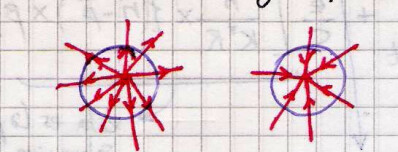
\includegraphics[width=0.4\textwidth]{images/fig_ft1_radiacion_esferica_no.jpg}
 
 Una corriente $J\hat{r}$ no produce \vb{B} y se tienen
 \[
	\vb{B}^0_{rad} = \frac{k^2}{r}( \hat{r} \times \vb{p} ) \euler^{ikr} \qquad \qquad 
	\vb{E}^0_{rad} = \frac{k^2}{r}( \hat{r} \times \vb{p} ) \euler^{ikr} \times \hat{r}
 \]
	\begin{figure}[htb]
		\begin{center}
		\includegraphics[width=0.4\textwidth]{images/fig_ft1_pot_irrad2.pdf}	 
		\end{center}
		\caption{Estado de polarización del campo de radiación.}
	\end{figure} 
 \item Para que un campo sea de radiación debe tener flujo \vb{S} no nulo en el infinito.
 Si los campos van como $1/r$ entonces el Poynting va como $1/r^2$ y $dS$ va como $r^2$
 de modo que $\langle\vb{S}\rangle \cdot d\vb{S}$ tiene valor constante (un flujo que se
 va y no retorna a la fuente). Si el campo va como $1/r^2$ y entonces no produce flujo
 lejos.
 \item Si hacemos la aproximación $\ell=1$ en $\sum_\ell$ resulta que se obtiene un momento
 magnético oscilante más un cuadrupolo eléctrico.
 \item La radiación a orden $\ell=0$ es un dipolo eléctrico oscilante (ver figura)
	\begin{figure}[htb]
		\begin{center}
		\includegraphics[width=0.4\textwidth]{images/fig_ft1_pot_irrad3.pdf}	 
		\end{center}
		\caption{}
	\end{figure} 
 \item La distribución angular de potencia para la parte cuadrupolar que surge con $\ell=1$ es
	\[
		\left\langle\dtot{P}{\Omega}\right\rangle = \frac{ck^6}{128\pi} Q_0^2 \sin(\theta)^2 
\cos(\theta)^2
	\]
	que es para una fuente con simetría de revolución.
	\[
		\vm{ \dtot{P}{\Omega} } = \frac{ck^6}{128\pi} |\hat{r} \times \vb{Q} |^2, 
	\]
	donde $\vb{Q}$ es un vector que vale $\hat{n} \cdot \overline{Q}$, o bien indicialmente $n_iQ_{ij}$.
\end{itemize}

\subsection{Radiación a orden $\ell=1$}

La aproximación siguiente, $\ell=1$, corresponde a
\[
	\vb{A}(\vbx) = \frac{4\pi}{c} i k \sum_{m=-1}^{1}
	h^{(1)}_\ell(kr) Y_{1 m}(\theta,\vp)
	\int_V \vb{J}(\vbx') j_1(kr') Y_{1 m}^*(\theta',\vp') d^3x' 
\]
donde utilizamos
\[
	j_1(kr') = \frac{kr'}{3} \qquad 
	Y_{11} = - \sqrt{ \frac{3}{8\pi} } \: \sin\theta \: \euler^{i \phi} \qquad 
	Y_{10} = \sqrt{ \frac{3}{4\pi} } \: \cos\theta 
\]
\[
	Y_{1,-1} = (-1)^{1} Y_{11}^* = \sqrt{ \frac{3}{8\pi} } \: \sin\theta \: \euler^{-i \phi} 
\]
e introduciéndolo en la cuenta anterior,
\[
	\vb{A}(\vbx) = \frac{ i k^2 }{ 2 c } h^{(1)}_1(kr) \left[ 
	 \int_V \vb{J}(\vbx') r' 2 \left( \sin\theta \: \euler^{-i \phi} \: \sin\theta'\:\euler^{i\phi'} +
	\cos\theta\cos\theta' \right) \right] d^3x'  
\]
pero este término se puede dividir en dos: (1) momento dipolar magnético oscilante y (2) cuadripolo
eléctrico.

\notamargen{Flujo de Poynting no nulo en el $\infty$ caracteriza un campo de radiación, entonces
tenemos energía que se va y no retorna.}

El corchete (yo junté dos términos que parecían ser iguales -al menos como estaban copiados-) da una cosa
como
\begin{multline*}
	[..] = 2 (\sin\theta\sin\theta'[\cos\vp\cos\vp' + \sin\vp\sin\vp'] + \cos\theta\cos\theta') = \\
	2 \frac{\pe{x}{x'}}{|\vbx||\vbx'|} = 2 \rver\cdot\frac{\vbx'}{|\vbx'|}, 
\end{multline*}
tras lo cual se transforma el integrando
\[
	\vb{A}(\vbx) = \frac{ i k^2 }{ c } h^{(1)}_1(kr) \int_V \vb{J}(\vbx') ( \nver \cdot \vbx' ) \: d^3x'
\]
y usando la identidad del doble vectorial product ID 2b para el producto escalar en el integrando,
podemos escribir
\[
	\vb{J}(\pe{\nver}{x'}) = \frac{1}{2}
	\left[ \vb{J} (\pe{\nver}{x'}) + \vbx' (\pe{\nver}{J}) \right]
	\frac{1}{2}( \pv{x'}{J} ) \times \nver
\]
pero recordando el momento dipolar magnético
\[
	\pv{m}{\nver} = \frac{1}{2c} \int (\pv{x'}{J}) d^3x \times \nver,
\]
podemos descomponer las contribuciones en dos:
\[
	\vb{A}^{\ell=1}(\vbx) = \vb{A}^{\ell=1}_m(\vbx) + \vb{A}^{\ell=1}_Q(\vbx),
\]
contribuciones magnética y cuadrupolar.
Considerando esta separación, serán
\[
	\vb{A}^{\ell=1}_m(\vbx) = i k^2 h_1^{(1)}(kr) \pv{m}{\nver}, 
\]
donde $h_1^{(1)}$ es el campo lejano visto y el campo magnético correspondiente surge de tomarle
rotor a esta expresión.
Reciclando cálculos anteriores y quedándonos solamente con aquello que aporta a la radiación
\[
	\vb{B}^{\ell=1}_m(\vbx) = k^2 (\pv{\nver}{m}) \times \nver \frac{\euler^{ikr}}{r}
\]
Luego, dado que la relación del campo $\vb B$ con el campo eléctrico es a través de un rotor,
se tiene que $ \rotorm{E}^{\ell=1} \sim \rotorm{A}^{\ell=1} $ y entonces los campos mismos
son similares si sus divergencias son iguales, i.e. si
\[
	\divem{E}^{\ell=1} \sim \divem{A}^{\ell=1}
\]
entonces por el teorema de Helmholtz y lo anterior se tiene
\[
	\vb{E}^{\ell=1} \sim \vb{A}^{\ell=1}.
\]
En efecto, se tiene
\[
	\vb{E}^{\ell=1} = i k \vb{A}^{\ell=1} = 
	- \frac{1}{c}\dpar{\vb A}{t}_m^{\ell=1} - \nabla\phi_m^{\ell=1} 
\]
de manera que tiene que ser $\phi_m^{\ell=1} = 0$ en todo el espacio, porque justamente
la derivada de $\vb A$ es el segundo término.

Las expresiones son iguales a las de un dipolo eléctrico oscilante; podemos concluir que
\[
	\vm{\dtot{P}{\Omega}} = \frac{c}{8\pi} k^4 |\vb m|^2 \sin^2\theta
\]
siendo la diferencia dada por la polarización.
Finalmente,
\[
	\vb{A}^{\ell=1}_m(\vbx) = i k \pv{m}{\nver}\frac{\euler^{ikr}}{r} 
	\left( 1 - \frac{1}{ikr} \right). 
\]
Como se tiene $\divem{E}=0$ por estar fuera de la fuente debe ser $\divem{A}=0$.
Entonces se requerirá que el orden 1 cúmplala.
Usaremos la identidad ID 5 previa reescritura abreviada de $\vb m f(r)$ donde el factor
$f(r)$ tiene todo lo que acompaña en la expresión de $\vb A$. Entonces
\[
	\divem{A}^{\ell=1}_m = - \nver \cdot [ \Nabla f \times \vb m],
\]
pero como $\Nabla f$ es proporcional a $\nver$ que es a su vez paralelo a $\rver$ se
tendrá que el producto escalar indicado es nulo.

La potencia total irradiada es
\[
	P = \frac{c k^4}{3} |\vb m|^2.
\]

Ahora retomamos el término cuadrupolar, que es
\[
	\vb{A}^{\ell=1}_Q(\vbx) = \frac{\euler^{ikr}}{2cr} \left( \frac{1}{r} -ik \right)
	\int \left[ ( \pe{\nver}{x'} ) \vb J + \vbx' ( \pe{\nver}{J} ) \right] d^3x'
\]
pero lo trabajaremos con una sola componente para simplificar el análisis,
\[
	{A^{\ell=1}_i}_Q(\vbx) = -\frac{ik\euler^{ikr}}{2cr} \left( 1 - \frac{1}{ikr} \right)
	n_i \int \left[ x_i' \vb J + \vbx' J_i \right] d^3x'
\]
y notemos que la divergencia de un tensor de tercer rango da
\[
	\partial_k'( x'_i x'_j J_k ) = x'_i J_j + x'_j J_i + x'_i x'_j \Nabla'\cdot \vb{J}
\]
la cual si integramos y aplicamos teorema de la divergencia se ve que es nulo.
\[
	\int (x'_iJ_j + x'_jJ_i) d^3x = -\int x'_i x'_j \Nabla'\cdot \vb{J} \: d^3x =
	-i\omega \int x'_i x'_j \rho(\vbx') \: d^3x
\]
Luego,
\[
	{A_j}_Q^{\ell=1} = - \frac{k^2}{2} \frac{\euler^{ikr}}{r} \left( 1 - \frac{1}{ikr} \right)
	\int \: x'_j (\pe{\nver}{x'}) \rho(\vbx') \: d^3x'
\]

Ahora deberíamos hacer $ \vb B = \nabla \times \vb{A}_Q$, pero tendremos en cuenta
solamente los términos de radiación tirando a la basura el resto. Siempre bajo la
rule: $ \nabla\times \equiv i k \nver \times $ se tiene la cadena
\[
	\nabla \times \vb{A}_Q = i k \nver\times \vb{A}_Q \qquad \qquad 
	\vb E_Q = \frac{i}{k} \rotorm{B} = \pv{B}{\nver}
\]
y vemos que tal como se cumple con la radiación en el vacío se tienen campos $\vb E \perp \vb B$
y de igual módulo. Entonces
\[
	\vb{B}_Q(\vbx) = - \frac{ik^3}{2} \frac{\euler^{ikr}}{r} \nver \times
	\int \vbx' (\pe{\nver}{x'}) \rho(\vbx') \: d^3x'
\]
Recordando la definición del momento cuadrupolar, convertimos $Q_i \equiv n_j Q_{ij}$ en su
correspondiente expresión vectorial
\[
	\nver \times \vb{Q} = 3 \nver \times \int \vbx' (\pe{\nver}{x'}) \rho(\vbx') \: d^3x'
\]
Luego, para solamente el campo de radiación se tendrá
\[
	\vb{B}_Q^{\ell=1} = - \frac{ik^3}{6} \frac{\euler^{ikr}}{r} \nver \times \vb{Q} \qquad 
	\qquad \vb E = - \nver \times \vb B
\]

Calculando el Poynting promedio se llega a
\[
	\vm{\vb S} = \frac{c}{8\pi} |\vb B|^2 \nver 
\]
y
\[
	\vm{ \dtot{P}{\Omega} } = \frac{ck^6}{288\pi} |\nver \times \vb Q|^2
\]

Caso particular: fuente con eje de simetría de revolución. En este caso podemos definir ejes
principales para el tensor y recordando su traza nula
\[
	Q_{33} \equiv Q_0 \qquad Q_{22} = Q_{11} = - \frac{1}{2}Q_0
\]
para un versor $\nver = (n_1, n_2, n_3)$ siendo estos ejes $1,2,3$ ejes principales será
\[
	\vb{Q} = (Q_{11}n_1, Q_{22}n_2, Q_{33}n_3)
\]
\notamargen{Ojo que acá aparece $Q$ vector además del tensor $Q$.}
o bien $Q_i = Q_{ij}n_j$ de modo que $\vb{Q} = Q\cdot\nver$ y, luego de un poco de álgebra,
\[
	|\nver \times \vb Q|^2 = \Frac{3Q_0}{2} (n_2^2n_3^2 + n_1^2n_3^2)=
	\Frac{3Q_0}{2} \sin^2\theta \cos^2\theta
\]
que es una expresión que no depende de $\vp$ como era de esperar por la simetría de revolución.
Los versores $n_j$ se expresaron en esféricas (ver apéndice).
Entonces
\[
	\vm{ \dtot{P}{\Omega} } = \frac{ck^6}{128\pi} Q_0^2 \sin^2\theta \cos^2\theta 
\]
y hemos hecho una aproximación para orden $\ell=1$. Volvemos a poner el pic que ya aparece
antes,

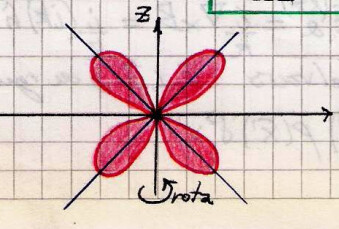
\includegraphics[width=0.25\textwidth]{images/fig_ft1_trebol_4hojas.jpg}

\[
	\vb{A} = \frac{1}{cR} \dot{\vb{p}}(t') + \frac{\dot{\vb{m}}(t')}{cR} \times \hat{n} + 
	\frac{1}{6c^2R} {\overline{Q}}(t') \cdot \hat{n}
\]
que es la radiación dipolar eléctrica,  magnética y cuadrupolar eléctrica.

\begin{ejemplo}{\bf Sinopsis de radiación}

De la sinopsis de radiación destaco
\[
	A_\mu(\vbx,t) = \frac{1}{c} \int \: \frac{J_\mu(\vbx',t')}{|\vbx-\vbx'|} 
	\delta\left( t' + \frac{|\vbx-\vbx'|}{c} - t \right) \: d^3x dt'
\]
y para carga puntual
\[
	\phi(\vbx,t) = e \left| \frac{1}{kR} \right|_\text{ret} \qquad \qquad 
	\vb{A}(\vbx,t) = \frac{e}{c} \Frac{\vb{u}}{kR}_\text{ret}
\]
y campo eléctrico de una partícula cargada
\[
	\vb{E}(\vbx,t) = e \left[ \frac{ (\nver -\vb{\b} ) \cdot ( 1 - \beta^2 ) }{ k^2 R^2 } \right]_\text{ret} +
	\frac{ e }{ c } \left[ \frac{ \nver }{ k^3 R } \times \{ ( \nver - \vb{\b} ) \times \vb{\b} \} \right]_\text{ret}
\]
el segundo término es un campo de aceleración, y el corchete $[...]$ es la parte que sobrevive
a grandes distancias.
\[
	\vb{B}(\vbx,t) = \nver \times \vb{E}(\vbx,t).
\]
 
\end{ejemplo}



\begin{ejemplo}{\bf Problema 10}

Estamos haciendo la aproximación de que cualquier punto sobre la flecha roja tiene el mismo
tiempo retardado, ver ilustración debajo.
\[
	z(t') = a \cos( \omega t' )
\]
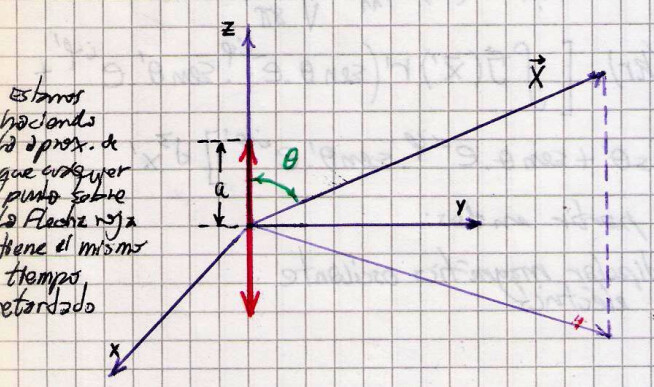
\includegraphics[width=0.45\textwidth]{images/fig_ft1_antena_probl.jpg}

\[
	R = | \vbx - \vb{r}(t_\text{ret}) | \qquad 
	\nver = \frac{ \vbx - \vb{r}(t_\text{ret}) }{| \vbx - \vb{r}(t_\text{ret}) |}
\]
luego si $|\vbx|\gg a$ es $ R \sim |\vbx| $ y $ \nver \sim \vbx/|\vbx|$
\[
	t'= t_\text{ret} = t - \frac{R(t_\text{ret}))}{c}
\]
\[
	k = 1 - \nver\cdot\vb{\b}(t_\text{ret})
\]
Resultan además
\[
	\vb{x}(t') = a \cos(\omega t') \zver \qquad \qquad 
	\vb{\b}(t') = - \frac{\omega a}{c} \sin(\omega t')\zver
\]
\[
	k = 1 + \frac{a\omega}{c}\sin(\omega t')\sin\theta
\]
\[
	|\nver\times(\nver\times\vb{z})| = \sin\theta
\]
y la energía saliente respecto al tiempo 
\[
	\dtot{\mathcal{E}}{t} = dP = \frac{c}{4\pi} | R \vb{E}_a |^2 \: d\Omega
\]
Poynting da el flujo en tiempo $t$ pero necesitamos respecto a $t'$.
\[
	1 = \frac{t}{t'} - \frac{1}{c} \nabla\vb{R} \left( \dtot{\vbx}{t'}(t') \right)
\]
donde en el producto escalar el primero es $\nver$ y el segundo $\vb u$. Luego,
\[
	\dtot{P}{\Omega}|_{t'} = \frac{ c }{ 4 \pi } \Frac{e}{c}^2 
	\frac{[ \nver \times {\nver - \vb{\b}}\times\vb{\b}]}{k^5}
\]
\[
	\dtot{P}{\Omega}|_{t'} = \frac{ e^2 }{ 4 \pi c}
	\frac{ \sin^2\theta \omega^4 a^2 \cos^2(\omega t')}
	{[ 1 + \omega_0 a/c \sin(\omega t')\cos\theta ]^5}
\]
con $\beta = \omega_0 a / c $ y entonces
\[
	\dtot{P}{\Omega}|_{t'} = \frac{ e^2 c^2 B^4}{4 \pi a^2}
	\frac{\sin^2\theta  \cos^2(\omega t')}	{[ 1 + \omega_0 a/c \sin(\omega t')\cos\theta ]^5}
\]
y 
\[
	\vm{ \dtot{P}{\Omega}|_{t'} }
\]
es la integral de la guía [cualquier cosa que eso signifique]. Caso relativista.

\end{ejemplo}

\subsection{Radiación dipolar eléctrica y magnética y cuadrupolar eléctrica}

Véase la figura para entender la nomenclatura de cosas. Suponemos que $ R \gg a $, donde $a$ es el 
tamaño de la fuente localizada. Consideramos $ t_\text{ret} = t - |\vb{R} - \vbx|/c$ el tiempo que
le toma a la radiación ir de $\vbx$ a $\vb{R}$.

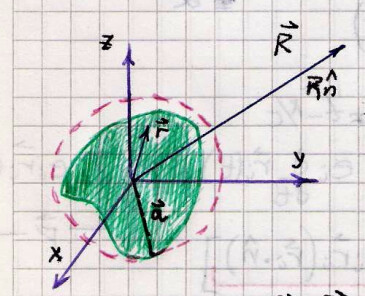
\includegraphics[width=0.3\textwidth]{images/fig_ft1_rad_dipolar_cuadrupolar.jpg}

\[
	\vb{A}(\vb{R},t) = \frac{1}{c} \int \frac{ \vb{J}(\vb{r},t_\text{ret})}{|\vb{R}-\vb{r}|} \: dV
\]
\notamargen{Acá uso $\vb r$ porque estaba así la carpeta pero luego moveré todo a $\vb x$
vector dado que es mi convención usual.}
Las aproximaciones de la distancia llevan a
\[
	|\vb{R} -\vb r | = \sqrt{ R^2 \left( 1 - 2 \frac{1}{r^2}\pe{r}{R} + \Frac{r}{R}^2 \right) } 
	\sim \left( 1 - \frac{\pe{r}{R}}{R^2} \right) R = R - \pe{r}{\nver}
\]

Como el campo eléctrico y magnético son perpendiculares y en módulo iguales sólo me calentaré
por $\vb A$ y dentro de éste solamente por el campo que dará radiación. Es decir,
\[
	\vb{A}(\vb{R},t) = \frac{ 1 }{ c R } \int \vb{J}(\vb r,t') \: dV
\]
En la expansión
\[
	\Nabla\times\frac{\vb a}{R} = \Nabla\Frac{1}{R} \times\vb a + \frac{1}{R} \rotorm{a}
\]
me quedo sólo con el último término ya que el primero da algo que va como $1/R^2$. El que
sobrevive, será
\[
	\rotorm{a}(t') = \Nabla t' \times \dtot{\vb a}{t'}
\]
Y como $ t' = t - R/c + \pe{\nver}{r} / c $ su gradiente  será $ \Nabla t' = - \nver/c + \sigma(1/R)$
pero no los quiero.
\[
	\vb{B}_\text{rad} = \rotorm{A} = - \frac{1}{c} \nver \times \vb A
\]

Estamos en $\lambda$ muy grandes respecto a la dimensión de las fuentes, se hace un Taylor en torno
a $t_r \equiv t - R/c$
\[
	\vb{J}(\vb r,t_\text{ret}) \approx \vb{J}(\vb r,t_r ) + 
	\left. \dpar{\vb J}{t}\right|_{t_r-t-R/c} - \frac{\pe{\nver}{r}}{c}
\]
donde el primer término del rhs es el que generará radiación dipolar eléctrica y como
\[
	\left| \dpar{\vb J}{t} \frac{\pe{\nver}{r}}{c} \right| \ll |\vb J|
\]
y en el caso armónico con $ \omega a / c \ll 1$ se construye
\[
	\vb{A}(\vb{R},t) \approx \frac{ 1 }{ c R } \int \vb{J}(\vb r,t_r) \: dV
	+ \frac{ 1 }{ c R } \dtot{}{t_r} \int \vb{J}(\vb r,t_r) \frac{\pe{\nver}{r}}{c} \: dV
\]
Defino por conveniencia algunas cosas:
\[
	\vb M = \frac{1}{2c} \pv{r}{J} \qquad 
	\pv{\nver}{M} = \frac{1}{2c} \nver\times( \pv{r}{J}) =
	\frac{1}{2c} \left[ \vb{r}(\nver\cdot\vb J) - \vb{J}(\nver\cdot\vb r)\right]
\]
donde el corchete en el rhs es $\alpha$ o bien la reescritura
\[
	\pv{\nver}{M} =  \frac{1}{2c} \left[ \vb{r}(\nver\cdot\vb J) + \vb{J}(\nver\cdot\vb r)\right]
	- \frac{1}{c} \vb{J}(\nver\cdot\vb r)
\]

Ahora trabajaremos con cargas puntuales y defino $t'= t_r $ de manera que
\[
	\int \vb{J}(\vb r,t') \: dV = \dtot{}{t}( \sum e_i \vb{r}_i(t') )
\]
y para $\a$ se tiene
\[
	\a = \sum_i e_i \left[ \vb{r}_i (\nver\cdot\vb{M}_i) + \vb{\mu}_i(\vb{r}_i\cdot\nver) \right]=
	\dtot{}{t}\left[ \sum e_i \vb{r}_i( \vb{r}_i\cdot\nver )\right]
\]
y ahora tiene la pinta de cuadripolo lo que está dentro del corchete en el extremo del rhs.
Le puedo agregar algo en la dirección $\nver$ y no cambio el campo,
\[
	\a' = \dtot{}{t'} \left[ \sum e_i 3 \vb{r}_i( \vb{r}_i\cdot\nver) - \nver r^2_i \right] \frac{1}{3}
\]
y será
\[
	\a'= \frac{1}{3} \dtot{}{t'} Q(t')\cdot\nver
\]
donde $Q_{ij} = \sum_i e_i( 3 x_jx_k - \delta_{jk}r_i^2)$.
Tenemos
\[
	\vb{A} = \frac{1}{cR} \dot{\vb{p}}(t') + \frac{\dot{\vb{m}}(t')}{cR} \times \hat{n} + 
	\frac{1}{6c^2R} {\overline{Q}}(t') \cdot \hat{n}
\]
Luego, los campos de radiación serán
\[
	\vb{B}_\text{rad} = \frac{1}{c^2R}
	\left[ 
	\ddot{ \vb{p} } \times \nver + \frac{1}{cR} (\dot{\vb m}(t')\times\nver) \times \nver + 
	\frac{1}{6c} ( \dddot{Q}(t')\cdot\nver )\times \nver 
	\right]
\]
\[
	\vb{E}_\text{rad} = \frac{1}{c^2R}
	\left[ 
	( \ddot{ \vb{p} } \times \nver ) \times \nver + 
	\nver \times \ddot{\vb m} +
	\frac{1}{6c} \{ ( \dddot{Q}(t')\cdot\nver )\times \nver \}\times \nver
	\right]
\]

Veamos algunas aplicaciones de esta teoría desarrollada.
Suponiendo radiación dipolar eléctrica,
\[
	\vb{P}(t') = \vb{P}_0 \euler^{ - i \omega t }
\]
la aceleración
\[
	\ddot{ \vb{P} }(t') = - \omega^2 \vb{P}_0 \euler^{ - i \omega t }
\]
de modo que para el campo magnético de radiación se tiene 
\[
	\vb{B}_\text{rad} = \frac{\omega^2}{c^2R} \vb{P}_0\times\nver \euler^{i \omega R/c} \euler^{ - i \omega t }
	\sim - \frac{\omega^2}{c^2} \frac{ \vb{P}_0\times\nver }{R}
\]
luego,
\[
	\vm{ \dtot{P}{\Omega} } = \frac{ \omega^4 }{ 8 \pi c^3 } P_0^2 \sin^2\theta
\]
y la potencia emitida en todo ángulo será
\[
	\vm{P} = \frac{ \omega^4 }{ 3 c^3 } P_0^2.
\]

Para la radiación dipolar magnética, será
\[
	\vb{m} = \vb{m}_0 \euler^{ - i \omega t },
\]
y las cuentas son las mismas con el reemplazo obvio,
\[
	\vm{ \dtot{P}{\Omega} } = \frac{ \omega^4 }{ 8 \pi c^3 } m_0^2 \sin^2\theta,
\]
\[
	\vm{P} = \frac{ \omega^4 }{ 3 c^3 } m_0^2.
\]


\subsection{Ejemplo de antena}

Consideramos un generador de radiofrecuencia (de onda) y ponemos como condición de contorno
para la corriente un nodo en cada extremo de la antena.
La parte temporal es siempre $\euler^{i \omega t}$.

Sea una pequeña antena de longitud $d$ (ver figura) tal que 
\[
	\vb{J}(\vb{x}') = I \sin( k[d/2 - |z|] ) \delta(x') \delta(y')  \hat{z}
\]
que tiene nodos de la corriente en los extremos. Luego considerando fuente armónica ($A=A(x)\exp(i\omega t)$)
será
\[
	\vb{A}(\vb{x}) = \frac{1}{c} \int_V' \frac{ \vb{J}(\vb{x}') \euler^{ i k |\vb{x}-\vb{x}'| }}
	{ |\vb{x}-\vb{x}'| } dv'
\]

\begin{figure}[htb]
	\begin{center}
	\includegraphics[width=0.3\textwidth]{images/fig_ft1_antena.pdf}	 
	\end{center}
	\caption{}
\end{figure} 

Hacemos algunas aproximaciones geométricas de distancia amparadas en la figura de más abajo porque
solo calcularemos para la zona de radiación.
	
\begin{figure}[htb]
	\begin{center}
	\includegraphics[width=0.4\textwidth]{images/fig_ft1_antena2.pdf}	 
	\end{center}
	\caption{}
\end{figure} 

Estas aproximaciones son clásicas de los problemas de difracción.
\[
	|\vb{x}-\vb{x}'| = \sqrt{ x^2 + x'^2 - 2xx'\cos(\theta)} =  
	x( 1 - 2x'/x \cos(\theta) + (x'/x)^2)^{1/2} 
\]
y quedándonos a primer orden,
\[
	|\vb{x}-\vb{x}'|\approx x (1 - x'/x \cos(\theta))
\]
de manera que aceptamos una buena aproximación y una bruta,
\[
	|\vb{x}-\vb{x}'| \approx x - x' \cos( \theta ) \qquad \qquad |\vb{x}-\vb{x}'| \approx x
\]
para así escribir
\[
	\approx \frac{1}{|\vb{x}|} \euler^{ikx} \euler^{-ikx'\cos(\theta)}
\]
donde notamos que hemos aproximado de una forma dentro del argumento de la exponencial compleja
y de otra en el denominador de la fracción.

Así, resulta
\[
	\vb{A}(\vb{x}) = \frac{1}{c} \frac{\euler^{ i k x} }{x} \int_V' \vb{J}(\vb{x}') 
		\euler^{ i k x' \cos(\theta) } dv'
\]

Existe condición de contorno que en los extremos la corriente debe ser nula, entonces debe haber nodos
del seno (en $\pm d/2$) y los $d$ posibles son $ n\lambda/2$.
\[
	\vb{A}(\vb{x}) = \hat{z} \frac{2I\euler^{ikx}}{ckx}\left[ \cos( kd/2 \cos(\theta) )- 
		\cos( kd/2 ) \right]\frac{1}{\sin(\theta)^2}
\]
y este resultado para el $\vb A$ de la integración sirve para los tres casos que nos interesarán.
Vemos que es paralela a la antena
Entonces, pasando a esféricas
\[
	\vb{A}(\vb{x}) = A_z \hat{z} \qquad \qquad \vb{A}(\vb{x}) =  A_z\cos(\theta)\rver - 
		A_z\sin(\theta) \thetaver
\]
Los campos $\vb E, \vb B$ están en fase, $\vb E \propto \vb B$, son transversales entre sí y con
la dirección de propagación. Además, van como $ 1 / r $.
La potencia será
\[
	\vm{ \dtot{P}{\Omega} } = r^2 \nver \cdot \vm{ \vb S } =
	\frac{I^2}{2\pi c} \Frac{\cos( kd/2 \: \cos\theta ) - \cos( kd/2 )}{\sin\theta}^2
\]
donde $\nver$ es un versor del punto de observación.


Entonces con $ kx' \ll 1$ (longitud de onda larga, $\lambda \gg d $) tenemos
\[
	\vm{ \dtot{P}{\Omega} } = \frac{I^2}{2c\pi} \Frac{kd}{2}^4 \sin^2 \theta
\]
identificando con $|\vb{p}| = Id^2/(2c)$ y este es el primer término multipolar.
El paréntesis es muy chico.

Con una antena de media longitud de onda ($kd=\pi$) ($\lambda/2=d$) es
\[
	\left\langle\dtot{P}{\Omega}\right\rangle=\frac{I^2}{2c\pi}\frac{\cos(\pi/2 
	\cos(\theta))^2}{\sin(\theta)^2}
\]
donde parece que usamos la aproximación del coseno de argumento pequeño,
\[
	\cos(x) \approx 1 - x^2.
\]

Finalmente, para una longitud de onda ($\lambda=2$ y $kd=2\pi$) se tiene 
\[
	\left\langle\dtot{P}{\Omega}\right\rangle=\frac{I^2}{2c\pi} \left[ \frac{ 2\cos(\pi/2 
	\cos(\theta))^2}{\sin(\theta)^2} \right]^2
\]
Las ilustraciones sucesivas de la figura \ref{fig_ft1_antena3} dan cuenta de estas diferentes longitudes.

\begin{figure}[htb]
	\begin{center}
	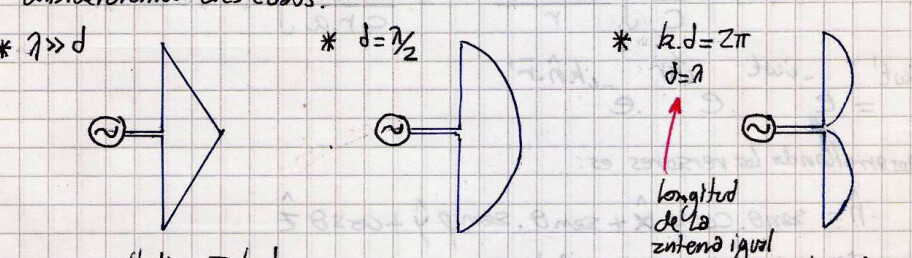
\includegraphics[width=1.0\textwidth]{images/fig_ft1_antena3.jpg}	 
	\end{center}
	\caption{Los tres casos que consideraremos.}
	\label{fig_ft1_antena3}
\end{figure} 


Como referencia tengamos en cuenta que las expresiones salen de 
\[
	\vb{B}_{rad} = -\frac{1}{c} \hat{n} \times \dot{\vb{A}} = ik \hat{n} \times \vb{A} 
\]
y
\[
	\vb{E}_{rad} = \vb{B}_{rad} \times \hat{n}
\]
Estas equivalencias son para campos de radiación nomás,
\[
	\vb{B}_{rad} = ik \hat{n} \times \vb{A} \qquad \qquad \vb{E}_{rad} = \vb{B}_{rad} \times \hat{n}
\]

\begin{ejemplo}{\bf Observación sobre la simetría azimutal}

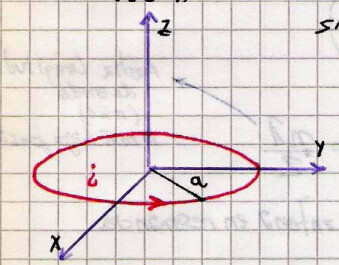
\includegraphics[width=0.4\textwidth]{images/fig_ft1_antena_sime_azimu.jpg}

\[
	\vb J = \frac{I}{c} \delta(r-a)\delta(\cos\theta) \phiver 
\]
que es la densidad de corriente para un anillo conductor. Luego
\[
	\vb A = \frac{Ia}{c} \frac{\euler^{ikr}}{r} \int_0^{2\pi}
	\euler^{ - i k a \sin\theta \cos\vp' } \: \cos\vp \: d\vp'
\]

La frecuencia de la corriente es la misma que la frecuencia de la radiación que se emite.
Como estamos haciendo una aproximación que involucra $ka$ no podemos calcular directamente
la integral sin realizar un taylor en $ka$.
Se debe tener $\lambda \gg a$ para que la corriente sea la misma.
 
\end{ejemplo}



\begin{ejemplo}{\bf Problema 3}
 
Resulta conveniente atacar por el $\vb A$ 

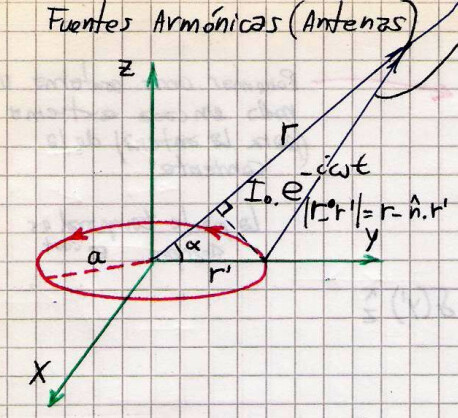
\includegraphics[width=0.4\textwidth]{images/fig_ft1_antena_problema3.jpg}

Dado el grafiquete es fácil ver que la corriente se debe poder escribir como
\[
	\vb{J}(\vbx,t) = \frac{I_0}{a}\delta(r-a)\delta(\cos\theta)\euler^{-i\omega t} \phiver
\]
Aproximando campo lejano
\[
	\vb{A}(\vbx,t) \approx \frac{I_0}{cra} \int \delta(r-a)\delta(\cos\theta) \euler^{-i\omega (t -|\vbx-\vbx'|/c)}
\]
que implica
\[
	\euler^{i\omega t'} = \euler^{-i\omega t} \euler^{ikr} \euler^{-i k \nver\cdot\vbx'}
\]
Desarrollando los versores se tienen
\[
	\nver = \sin\theta\cos\vp \xver + \sin\theta\sin\vp \yver + \cos\theta \zver
\]
\[
	\vbx' = a ( \cos\vp' \xver + \sin\vp' \yver )
\]
\[
	\nver \cdot \vbx' = a \sin\theta \cos(\vp-\vp')
\]
Luego, removiendo el approx pero recordando que es campo lejano,
\[
	\vb{A}(\vbx,t) =  \frac{I_0a}{cr} \euler^{i (kr-\omega t)} \int_0^{2\pi} 
	\euler^{-i k a \sin\theta \cos( \vp -\vp' )} \: d\vp' \: \vp'
\]
y como es simétrico, para cualquier $\vp'$ vale lo mismo (tomo $\vp=\pi$ ).
Entonces con ese valor
\[
	\vb{A}(\vbx,t) =  \frac{I_0a}{cr} \euler^{i (kr-\omega t)} \int_0^{2\pi} 
	\euler^{i k a \sin\theta \cos( \vp' )} \: \cos\vp' \: d\vp' \: (-\yver)
\]
Utilizando la expresión que define a las funciones cilíndricas de Bessel, será
\[
	\vb{A}(\vbx,t) = - \frac{aI_0}{2cr} \euler^{i (kr-\omega t)}
	\left[ 
	\frac{2\pi}{i} (-J_1(ka\sin\theta)) + 2\pi i J_1(ka\sin\theta)
	\right]
\]
donde se ha usado la propidad $ J_{-1} = -J_1 $. Finalmente,
\[
	\vb{A}(\vbx,t) = - \frac{aI_0}{cr} \euler^{i (kr-\omega t)}
	\: J_1(ka\sin\theta)) \: 2\pi \: \phiver
\]

Calculamos el campo magnético a través de la expresión simplificada y será
\[
	\vb B_{\text{rad}} = - \frac{1}{c} \nver \times \dot{\vb A} =
	\frac{2\pi ka I_0}{cr} \euler^{i(kr-\omega t)} \: J_1(ka\sin\theta)) \thetaver
\]
Consecuentemente, el campo eléctrico será
\[
	\vb E_{\text{rad}} = \vb B_{\text{rad}} \times \nver =
	-\frac{2\pi ka I_0}{cr} \euler^{i(kr-\omega t)} \: J_1(ka\sin\theta)) \phiver
\]
donde recordemos que en $ka=2\pi a/\lambda$ se halla la relación adimensional $\text{diam}/\lambda$
que nos permite caracterizar el campo lejano.
El flujo del Poynting será
\[
	\vm{\vb S} = \frac{1}{2c} \frac{\pi a^2}{r} k^2I_0^2 J_1(ka\sin\theta)^2 \rver.
\]

Aproximando $ 2 \pi a \ll \lambda $ se tiene
\[
	J_1(ka\sin\theta)) \approx \frac{ka}{2} \sin\theta,
\]
que viene de que $J_1(x)\approx x/2$ si el argumento es pequeño, y entonces el campo magnético
de radiación
\[
	\vb B_{\text{rad}} = \frac{k^2}{r} m_0 \euler^{-i\omega t} \euler^{ikr} \thetaver
\]
donde hemos definido
\[
	m_0 = \frac{1}{c}\pi^2 a I_0, \qquad \sin\theta\thetaver = (\nver\times\vb m)\times\nver
	\qquad \vb m = m_0\euler^{-i\omega t}\zver
\]
con lo cual llegamos a
\[
	\vb B_{\text{rad}} = \frac{k^2}{r} \: \euler^{ikr} \: (\nver\times\vb m)\times\nver.
\]

\end{ejemplo}

\begin{notas}{\bf Características relacionadas con antenas}
 
Tienen importancia la {\bf directividad} que está asociada a los ángulos de intensidad.
Se define
\[
	D = 4\pi r^2 \frac{\vm{S}}{\vm{P}},
\]
que mide la desviación respecto de un radiador isotrópico. La ganancia de la antena se mide
en dB y se define según
\[
	\text{Ganancia} = 10 \log_{10}(D) \; \text{dB}
\]

Se tiene por ejemplo $D=3/2 \sin^2\theta$ que da igual al dipolo eléctrico (se diferencia
por el estado de polarización). Ver gráfico

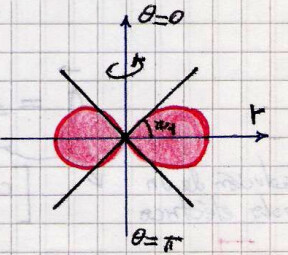
\includegraphics[width=0.2\textwidth]{images/fig_ft1_direct_antena_1.jpg}

Este gráfico tiene la simetría de revolución de la fuente.
Para otros valores [?], con $2\pi a/\lambda = 5\pi$ y, como vemos en la ilustración del
brillante artista, a medida que sube la frecuencia (y baja la longitud de onda) tenemos
lóbulos pequeños y surgen secundarios
 
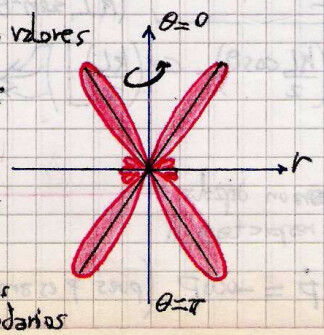
\includegraphics[width=0.2\textwidth]{images/fig_ft1_direct_antena_2.jpg}

Luego es importante la {\bf polarización}. Si la longitud de onda $\lambda$ es muy larga
tenemos polarización lineal

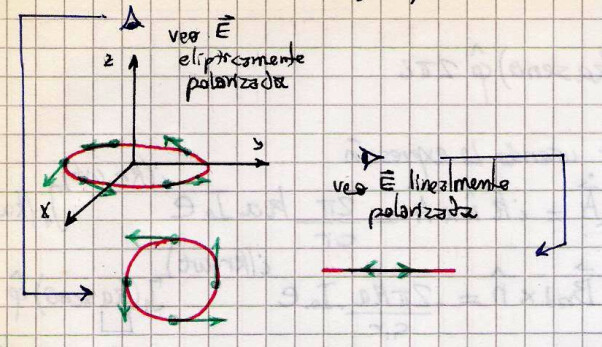
\includegraphics[width=0.45\textwidth]{images/fig_ft1_polarizacion_antena.jpg}

Finalmente, consideremos la {\bf resistencia de radiación},
\[
	\vm{P} = R_\text{rad} \: \frac{I_0^2}{2},
\]
que vendría a ser como la resistencia que hace el medio a que nosotros le hagamos transportar
una onda electromagnética a través de él.
En
\[
	\vm{S} = \frac{1}{2c} \frac{\pi a^2}{r^2} k^2 I_0^2 J_1(ka\sin\theta)^2
\]
y
\[
	\vm{P} = \frac{I_0^2}{2} \left[ \frac{\pi^2}{c} \Frac{2\pi a}{\lambda} 
	\int_0^{4\pi a/\lambda} \: J_2(u)\: du \right]
\]
identificamos el corchete como una $R_\text{rad}$.
 
\end{notas}

\begin{ejemplo}{\bf Problema 2}

La corriente se escribe
\[
	\vb J = I_0 \sin\left( kL /2 - k|z| \right)\delta(x) \delta(y)\euler^{-i \omega t} \zver
\]
y usando las aproximaciones de siempre
\[
	\vb{A} = \frac{ I_0 L }{ c r } \: \euler^{i(kr-\omega t)} 
	\left( \frac{ 2 }{ k L\sin^2\theta } \left[ \cos(kL\cos\theta/2) - \cos(kL/2) \right] \right)
\]
que se ve como el producto de la solución de un dipolo, el primer factor, y un factor de retardo
$F(kL/2,\theta)$, que es el factor dentro del paréntesis.

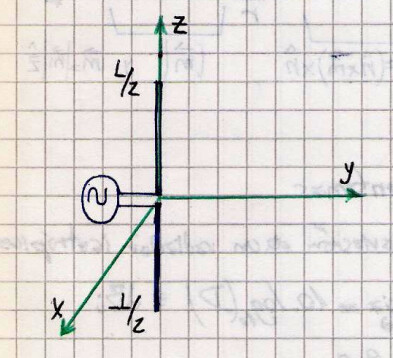
\includegraphics[width=0.4\textwidth]{images/fig_ft1_antena_prob2.jpg}

Téngase presente que para un dipolo con respecto a cierta longitud de onda $\lambda$ vale que
\[
	I_0L = - i \omega p \qquad \qquad \int JdV = \int J dS dz = I_0 L
\]
y luego como 
\[
	\rho v = \rho \dtot{z}{t}dV = \dtot{}{t}(\rho dV), 
\]
se tiene, pués $p$ es armónico, que
\[
	\dot{p} = - i \omega p
\]

Esto nos permite escribir entonces
\[
	\vb B_{\text{rad}} = i k \nver \times \vb A =
	i k \frac{I_0L}{cr} \euler^{i(kr-\omega t)} \: F(kL/2,\theta) \: (\nver\times\zver)
\]
\[
	\vb E_{\text{rad}} = \vb B_{\text{rad}} \times \nver =
	i k \frac{I_0L}{cr} \euler^{i(kr-\omega t)} \: F(kL/2,\theta) \: [(\nver\times\zver)\times \nver]
\]
\[
	\vm{S} = \frac{c}{8\pi} k^2 \Frac{}{}^2 \sin^2\theta F^2(kL/2,\theta)
\]

La antena es resonancia está caracterizada por $L = n\lambda/2$.
Luego, hay una condición de contorno de que en el extremo la corriente debe ser nula,
entonces debe haber nodos del seno lo cual lleva a que las posibles longitudes de
onda $\lambda$ deben ser múltiplos de $\lambda/2$.



\end{ejemplo}



% 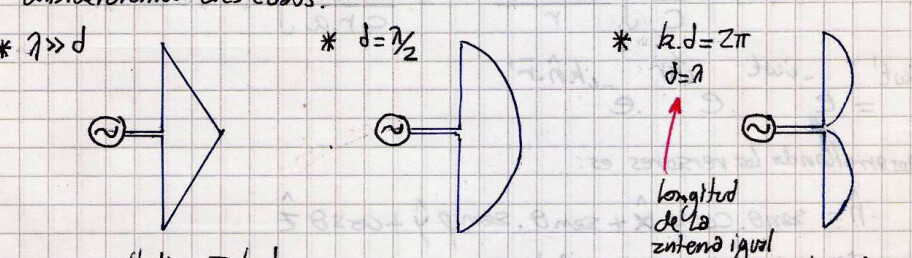
\includegraphics[width=1.0\textwidth]{images/fig_ft1_antena3.jpg}	

% =================================================================================================
\section{Campo de una partícula cargada en movimiento}
% =================================================================================================

Escribimos la densidad de corriente y la densidad de carga para una partícula
(con la delta de Dirac) según
\[
	\vb{J}(\vb{x}',t') = q\vb{v} \delta[ \vb{x}' - \vb{r}(t')]
\]
\[
	\rho(\vb{x}',t') = q \delta[ \vb{x}' - \vb{r}(t')]
\]
de manera que, introduciendo esta información en los potenciales retardados y, sin integrar,
se obtiene
\[
	\vb{A}(\vb{x},t) = \frac{1}{c} \int_{t'}\int_{V'} 
	\frac{ q\vb{v} \delta[ \vb{x}' - \vb{r}(t')] \delta[ t'-t +R/c] }{|\vb{x} -\vb{x}'|} dV' dt'
\]
\[
	\phi(\vb{x},t) = \frac{1}{c} \int_{t'}\int_{V'} 
	\frac{ q \delta[ \vb{x}' - \vb{r}(t')] \delta[ t'-t +R/c] }{|\vb{x} -\vb{x}'|} dV' dt'
\]
donde hemos usado $R\equiv |\vb{x}-\vb{x}'|$ de modo que es $R = R(t')$.
Luego de integrar en el espacio se obtienen
\[
	\vb{A}(\vb{x},t) = \frac{1}{c} \int_v' \frac{ q\vb{v} \delta[ t'-t +R/c] }{|\vb{x} -\vb{r}(t')|} dt' 
	\Rightarrow \vb{A}(\vb{x},t) = \left. \frac{q}{c} \frac{\vb{v}(t')}
	{(1-\hat{n}\cdot{\vb{\beta}})R(t')} \right|_{t'=t-R/c}
\]
\[
	\phi(\vb{x},t) = \frac{1}{c} \int_v' \frac{q \delta[ t'-t +R/c]}{|\vb{x} -\vb{r}(t')|} dt' 
	\Rightarrow \phi(\vb{x},t) = \left. \frac{q}{c} \frac{1}{(1-\hat{n}\cdot{\vb{\beta}})R(t')} 
	\right|_{t'=t-R/c}
\]
cuyas expresiones son los potenciales de Liènard-Wiechert. Hemos usado en las cuentas que 
\[
	\delta[t' - ( t - R(t')/c )] = \frac{1}{\dtot{}{t'}( t' + R(t')/c )} \delta( t-t')
\]
(idea que viene de $\delta f = (1/(df/dx_0)) \delta(x-x_0) $)\footnote{Que es propiedad de
la delta de Dirac y deberemos escribir de modo más adecuado.} y que 
\[
	R = |\vb{x}-\vb{x}'| = \sqrt{ x^2 + x'^2 - 2\pe{x}{x'} } \qquad \dtot{R}{t'} = 
	\frac{\dot{\vb{x}'}\cdot(\vb{x}-\vb{x}')}{R} = -\frac{\pe{R}{v}}{R} = -\hat{n}\cdot\vb{v}
\]
\[
	1 + \frac{1}{c} \dtot{R}{t'}  = 1 -\hat{n}\cdot\frac{\vb{v}}{c} = 1 - \hat{n}\cdot\vb{\beta}
\]
según la figura que ilustra bajo estas líneas

\begin{figure}[htb]
	\begin{center}
	\includegraphics[width=0.4\textwidth]{images/fig_ft1_campo_part_car.pdf}
	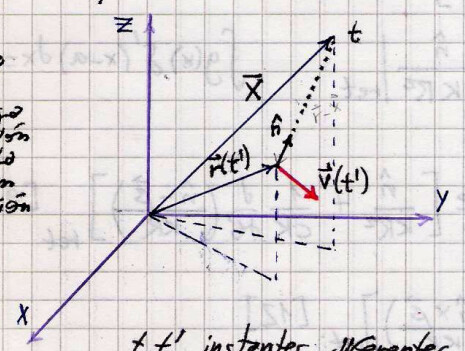
\includegraphics[width=0.4\textwidth]{images/fig_ft1_campo_part_carJPG.jpg}
	\end{center}
	\caption{}
\end{figure} 
\notamargen{Cuando evaluamos a tiempo $t$ donde llega la radiación la partícula se halla en otra
posición.}

Recordemos que $t,t'$ son instantes diferentes en un mismo sistema inercial.
Cuando la partícula está en $\vbx(t')$ emite y llega a $\vbx$ en $t$; momento en el cual 
$\vbx(t)$ es otro. La picture de la cosa vendría a ser algo como lo que se muestra abajo.

Las fuentes no dependen necesariamente de manera armónica del tiempo.

Es más fácil trabajar con las expresiones integrales antes de integrar en el tiempo.


Como los campos serán 
\[
	\vb{B} = \rotorm{A} \qquad \vb{E} = -\frac{1}{c}\dpar{\vb{A}}{t} - \Nabla\phi
\]
se tiene que 
\[
	\vb{E} = \left. q \frac{ (\hat{n}-\vb{\beta})(1-\beta^2)}{K^3R^2} \right|_{ret} + \left. 
	\frac{q}{c} \frac{\hat{n}\times[ (\hat{n}-\vb{\beta})\times \dot{\vb{\beta}} ]}{K^3R} \right|_{ret}
\]
donde se ve que vale $\vb{B} = \hat{n} \times \vb{E}$ que ya sabíamos para $\vb{E}_{rad}$ y $\vb{B}_{rad}$
y donde $K\equiv 1 - \hat{n}\cdot\vb{\beta} $

De acuerdo a la figura xxxx en $t'$ se produce el campo. Cuando la radiación llega a $\vb{x}$ en tiempo $t$ 
la partícula se halla en $\vb{x}'$ (tiempo $t$), de manera que la moraleja es que $t$ y $t'$ son instantes
de tiempo diferentes en un mismo sistema inercial.

\begin{figure}[htb]
	\begin{center}
	\includegraphics[width=0.3\textwidth]{images/fig_ft1_campo_part_car2.pdf}
	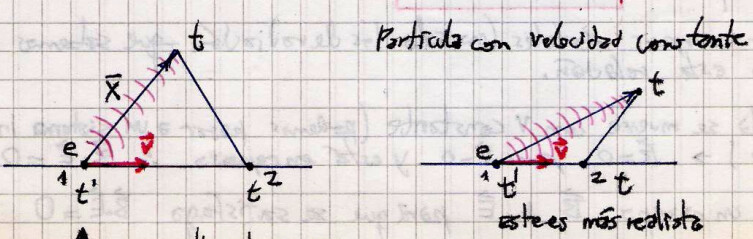
\includegraphics[width=0.6\textwidth]{images/fig_ft1_campo_part_car2JPG.jpg}
	\end{center}
	\caption{El campo se produce en $t'$ y la radiación llega cuando la partícula se halla
	en el punto 2.}
\end{figure} 

Ahora sigue un desarrollo un poco monster

\begin{ejemplo}{\bf Desarrollo cálculo campo}

Tenemos 
\[
	\vb A = \frac{e}{c} \int \frac{\vb v(t')}{R} \delta \: dt' \qquad \qquad 
	\phi = e \int \frac{1}{R} \delta \: dt'
\]
donde el argumento de la delta es $t'+ R/c -t$. Luego,
\[
	\nabla\phi = e \int \left[ \nabla\Frac{1}{R} \delta + \frac{1}{R} \nabla\delta \right] \: dt'
\]
Usamos
\[
	\nabla\delta = \delta'\nabla(t'+R/c-t) = \frac{\nver}{c}\delta'(t'+R/c-t)
\]
lo que nos permite
\[
	\nabla\phi = -e \int \frac{\nver}{R^2} \delta \: dt' + 
	e \int \frac{\nver}{R} \delta' \: dt'
\]
\[
	\frac{1}{c}\dtot{\vb A}{t} = - \frac{e}{c^2} \int \frac{\vb v}{R} \delta' \: dt' 
\]
\[
	\vb E = e \int \left[ \frac{\nver}{R^2} \delta + 
	\frac{1}{cR}(\vb{\beta} - \nver) \delta' \right] dt' 
\]
\[
	\vb B = \rotorm{A} = e \int (\nver\times\vb{\beta}) 
	\left[ -\frac{\delta}{R^2} + \frac{\delta'}{cR} \right] dt' 
\] 

La integral crucial parece ser
\[
	\int \frac{\nver}{R^2} \delta \: dt' = 
	\Frac{ \nver(t')/R^2(t') }{|d/dt'(t'+R/c)|}_{t' = t-R/c} =
	\Frac{\nver}{KR^2}_{\text{ret}}
\] 
donde usamos el colapso de la delta derivada (ver apéndice). 
\notamargen{Recordemos que $K \equiv \dtot{}{t'}( t' + R(t')/c )$.}
Expandiendo, resultan
\[
	\vb E = e \left[ \frac{\nver - \vb{\beta} }{K^2R^2} + \frac{\nver}{cK} \dtot{}{t'}\Frac{1}{kR}
	- \frac{1}{cK}  \dtot{}{t'}\Frac{\vb{\beta}}{kR} \right]_{\text{ret}}
\]
\[
	\vb B = e \left[ \frac{ \vb{\beta}\times\nver }{K^2R^2} 
	+ \frac{1}{cK} \dtot{}{t'}\Frac{\vb{\beta}}{kR}\times\nver \right]_{\text{ret}}
\]
\notamargen{Todas estas expresiones habría que chequearlas, doblechequearlas y triplechequearlas.}
 
 
\end{ejemplo}


Podemos sacar un par de frases importantes ya que 
\begin{itemize}
	\item Se puede ver que $\nver\times\vb E = \vb B$, lo cual vale también para 
	los campos totales, no solamente para los de radiación, como sabíamos.
	\item Si una partícula se mueve con $\vb{v}$ constante puedo pasar a un frame 
	inercial $S'$ donde es $\vb{v}=0$ y entonces $\vb{B}'=0$ de manera que como 
	$\pe{B}{E}=\pe{B'}{E'}=0$ se tiene $\vb{B}\perp\vb{E}$ en todo frame inercial
	(se las arregla para satisfacer eso).
	\item El $\vb{E}_{rad}$ estará dado por el $\vb{E}_a$.
	\item Toda partícula que está acelerada en un frame inercial debe irradiar ondas
	EM, entonces una partícula recorre una circunferencia (en un campo $\vb{B}$) si 
	aceptamos que lo que irradia es despreciable.
\end{itemize}

Sea ahora una partícula $e$ con $|\vb{v}|$ constante, entonces 
\[
	\vb{B}_{bs} = e\frac{\vb{\beta}\times\hat{n}}{\gamma^2k^3R^2} \;\; \text{(Lienard-Wiechert)}
	\qquad \qquad 
	\vb{B}_{bs} = e\frac{\vb{v}\times\hat{n}}{cR^2} \;\; \text{(Biot-Savart)}
\]
y 
\[
	\vb{E}_{v} = e\frac{ \hat{n}- \hat{\beta} }{\gamma^2k^3R^2}
\]
donde vemos que difieren en 
\[
	\frac{1-\beta^2}{(1-\hat{n}\cdot{\vb{\beta}})}.
\]

Tenemos entonces que
\[
	\vb{E}  = \vb{E}_v  + \vb{E}_a 
\]
que es un término de velocidad y uno de aceleración, estando los campos de radiación dados por
este último.
Toda partícula que se mueve con velocidad no constante en un sistema inercial debe radiar ondas
electromagnéticas.
Una partícula recorre una circunferencia en un campo $\vb B$ uniforme si aceptamos que lo que radía
es despreciable.

\begin{ejemplo}{\bf Partícula con velocidad constante}

Sea una partícula de carga $e$ con velocidad constante, será
\[
	\vb{B}(\vbx,t) = e \Frac{\beta\times\nver}{\gamma^2K^3R^2}_\text{ret}
\]
mientras que por Biot-Savart se tiene, con $\vb J = \rho \vb v = e \delta(\vbx'-\vbx)\vb v$ ,
\[
	\vb{B}_\text{BS} = \frac{e}{c} \frac{\vb v \times \nver }{R^3},
\]
que difieren en $\gamma^2K^3$ y dejamos de lado el retardo. La diferencia es despreciable.

Era de esperar que las expresiones difiriesen puesto que Biot-Savart es para corrientes
estacionarias y una carga con velocidad produce una corriente que no es estacionaria.
No obstante, si no radía, vemos que la aproximación es buena.
 
\end{ejemplo}


El campo de velocidad es 
\[
	\vb{E}_v = e \frac{(\hat{n}-\hat{\beta})}{\gamma^2(1-\hat{n}\cdot\vb{\beta})^3R^2} =
		e \left[ \frac{\vb{R}-R\vb{\beta}}{\gamma^2(1-\hat{n}\cdot\vb{\beta})^3R^2} \right]
\]
referidas las magnitudes a la figura \ref{fig_ft1_campo_carga_mov}. 
El ángulo $\beta$ es el que corresponde al punto $P$.

\begin{figure}[htb]
	\begin{center}
	\includegraphics[width=0.4\textwidth]{images/fig_ft1_campo_carga_mov2.pdf}
	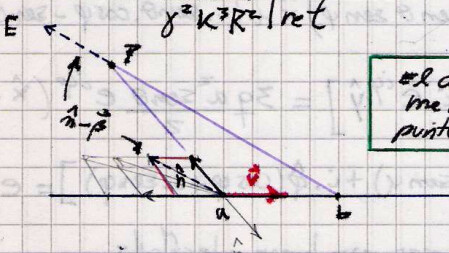
\includegraphics[width=0.4\textwidth]{images/fig_ft1_campo_carga_mov2JPG.jpg}
	\end{center}
	\caption{El campo en P me lo define un punto futuro b.}
	\label{fig_ft1_campo_carga_mov}
\end{figure} 

Desarrollamos en algún momento
\[
	r^2 = R^2 + \b^2R^2 - 2R^2\b\cos\theta = R^2(1+\b^2-2\b\cos\theta)
\]
que se conecta con
\[
	|\vb{E}_v| = e\frac{\sqrt{ R^2 + \beta^2 R^2 - 2R^2 \beta \cos(\theta)}}
		{\gamma^2( 1 - \vb{R}\cdot\vb{\beta}/R)^3 R^3} =
		e\frac{ [ \: 1 + \beta^2 - 2 \beta \cos\theta \: ]^{3/2}}
		{\gamma^2( 1 - \beta \cos\theta )^3 r^2}
\]
Queremos [?]
\[
	\dtot{ |\vb{E}_v| }{\theta}= 0,
\]
y ello significa que tiene que ser
\[
	3\b^2 ( 1 + \b^2 - 2\b \cos\theta )^{1/2} ( 1 - \beta \cos\theta )^2 
	\sin\theta (\cos\theta -1) = 0
\]
y analizamos factor a factor
\begin{itemize}
 \item $\sin\theta (\cos\theta -1) = 0$ implica por un lado $\sin\theta=0$ lo cual
 es un movimiento hacia adelante $(\theta=0)$ o hacia atrás $(\theta=\pi)$. El
 otro factor $\cos\theta = \pm 1$ da la misma información.
 \item $1 - \beta \cos\theta = 0$ implica $ \cos\theta = \b^{-1} > 1 $ y la 
 desechamos porque no puede ser.
 \item $1 + \b^2 - 2\b \cos\theta = 0$ corresponde a $|\vb E|=0$ y lleva a
	\[
		\frac{1 + \b^2}{2\b} = \cos\theta, 
	\]
	de modo que se desecha también.
 \item $\cos\theta - \b = 0$ es ``la condición''.
\end{itemize}

Entonces, con esta última condición $\cos(\theta) = \beta$ se tiene
\[
	\dtot{ |\vb{E}_v| }{\theta}= 0
\]
siendo los extremos $\theta=0,\pi$ que representan un movimiento hacia adelante o hacia atrás.
\[
	|\vb{E}_v(\cos\theta = \beta)| = \frac{e\gamma}{r^2}
\]
\[
	|\vb{E}_v(\cos\theta = 1)| = \frac{e (1+\beta^2-2\beta)^2}{R^2(1-\beta^2)^{-1}(1-\beta)^3}
\]
\[
	|\vb{E}_v{(\cos\theta = 1)}| = \frac{e }{R^2(1-\beta^2)^2 \gamma^2} = \frac{e}{r^2 \gamma^2}
\]
puesto que es $r=R(1-\beta)$. Vemos que, en ambos casos, es similar al campo estático pero con 
un factor corrector. Hacia adelante y hacia atrás el campo $\vb E$ se ve disminuido en un $1/\gamma^2$.

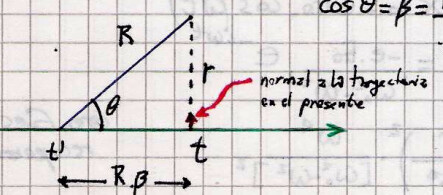
\includegraphics[width=0.4\textwidth]{images/fig_ft1_campo_carga_movJPG1.jpg}

En el figurin podemos ver que $\cos\theta=\b=R\b/R$ de la trigonometría.

En la Figura \ref{fig_ft1_campo_carga_mov} vemos que la longitud de las flechas es proporcional
a la intensidad del campo $\vb E$ en un dado punto presente.

\begin{figure}[htb]
	\begin{center}
	\includegraphics[width=0.4\textwidth]{images/fig_ft1_campo_carga_mov.pdf}
	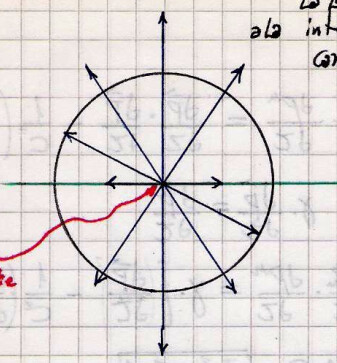
\includegraphics[width=0.3\textwidth]{images/fig_ft1_campo_carga_movJPG2.jpg}
	\end{center}
	\caption{campo de carga en movimiento}
	\label{fig_ft1_campo_carga_mov}
\end{figure}

Ahora consideraremos el campo eléctrico de las aceleraciones (el correspondiente a la radiación)
El campo de aceleración es
\[
	\vb{E}_a = \frac{e}{c} \frac{ \nver \times [ (\nver-\vb{\b})\times \dot{\vb{\b}} ]}{K^3 R} 
		\approx \frac{e}{c} \frac{ \nver \times ( \nver \times \dot{\vb{\b}})}{K^3 R} 
% 		= \frac{e}{c} \frac{}{K^3 R}
\]
donde usamos que $\b = v/c \ll 1$ y por ende $\nver-\vb{\b} \approx \nver$ y 
$ K = 1 - \pe{\nver}{\b} \approx 1$ (dos aproximaciones de orden consistente aunque parecen
no estar de acuerdo una cono otra) entonces es 
\[
	\nver \cdot \hat{\beta} \approx \nver
\]

Queremos ver la radiación de la partícula y al no haber dependencia temporal armónica no tomamos
el valor medio de manera que
\[
	\vb{S} = \frac{e^2}{4\pi c}\nver \left| \frac{\nver \times \dot{\vb{\b}}}{R}\right|^2
\]
donde no considero el \texttt{ret} porrque la velocidad es mucho menor a $c$.
\notamargen{Algunas de estas expresiones en la carpeta estaban evaluadas en \texttt{ret} y acá
no. Habría que justificar la explicación.}

% =================================================================================================
\section{Cálculo de potencia irradiada}
% =================================================================================================

Consideramos una partícula acelerada pero con velocidad no relativista.

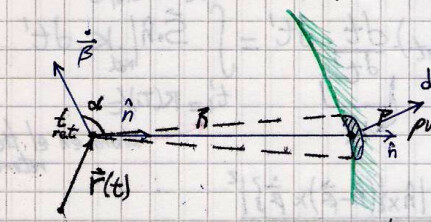
\includegraphics[width=0.5\textwidth]{images/fig_ft1_calculo_potencia_radiada.jpg}

Se realiza calculando el vector de Poynting,
\[
	\vb{S} = \frac{c}{4\pi} \pv{E}{B} = \frac{c}{4\pi} |\vb{E}_a|^2 \hat{n} =  \frac{e^2}{4\pi c}
		\hat{n} \left| \frac{\hat{n} \times \dot{\vb{\beta}} }{R} \right|^2
\]
Luego, siendo $\Omega$ el ángulo sólido subtendido por $d\nver$ desde $t_\text{ret}$ se tiene
\[
	dP = \vb{S}\cdot\hat{n} R^2 d\Omega =
		\frac{e^2}{4\pi c} \left| \hat{n} \times \dot{\vb{\beta}} \right|^2 d\Omega
\]
y entonces la potencia irradiada será
\[
	\dtot{P}{\Omega} = \frac{e^2}{4\pi c} \frac{\dot{v}^2}{c^2} \sin^2\theta = 
		\frac{e^2 \dot{v}^2 }{4\pi c^3} \sin^2\theta
\]
que depende del ángulo $\theta$  que en el dibujo de arriba es $\alpha$.

Luego, si integramos,
\[
	P = \frac{e^2 \dot{v}^2 }{4\pi c^3} \int\int \sin(\theta)^3 d\theta d\phi
	= \frac{2 e^2 \dot{v}^2 }{3 c^3}
\]
que es la fórmula de Larmor con $v/c \ll 1$. 

Ahora podemos prescindir de la restricción no relativista
usando que la $P$ es invariante lorentziano.
\[
	P = \frac{2 e^2}{3 c^3 m^2} \left( \dtot{\vb{p}}{t} \dtot{\vb{p}}{t} \right)
\]
y como $p_{\mu}( E/c , -\vb{p} )$ y $p^{\mu}( E/c , \vb{p} )$. 
\[
	-\dtot{p_\mu}{\tau} \dtot{p^\mu}{\tau} = \dtot{\vb{p}}{\tau} \dtot{\vb{p}}{\tau} - 
		\dtot{}{\tau}(E^2/c^2)
\]
donde recordemos que $E^2 = c^2p^2 + m^2c^4$,
\[
	\tau = \gamma (t-\beta x_\parallel) \qquad \qquad 
	\dtot{\tau}{t} = \gamma \qquad \Rightarrow \qquad 
	\dtot{\vb{p}}{\tau} \dtot{\tau}{t}= \gamma \dtot{\vb{p}}{\tau} = \dtot{\vb{p}}{t}
\]

Ahora querremos darle forma 3D a la potencia
\[
	P = - \frac{2}{3} \frac{ e^2 }{ m^2 c^3 } \dtot{P^\mu}{\tau} \dtot{P_\mu}{\tau} =
	\frac{2}{3} \frac{e^2\gamma^6}{c} \left[ \vb{\b}^2 - (\vb{\b} \times \dot{\vb{\b}})^2 \right]
\]
donde el resultado llega después de una cuenta un poco tediosa.
Luego,
\[
	\vb{S}\cdot\nver|_\text{ret} = 
	\frac{e^2 c}{4\pi} \left[ \frac{ \nver \times [ (\nver-\vb{\b})\times \dot{\vb{\b}} ]}{K^3 R}
	\right]_{\text{ret}}^2
\]
La potencia irradiada entre $t_1', t_2'$ conociendo su movimiento en dicho intervalo será
\[
	E = \int_{t_1=T_1+R(T_1)/c}^{t_2=T_2+R(T_2)/c} \: (\vb{S}\cdot\nver|_\text{ret}) \: K \: dt' =
	\int_{t_1'= R(T_1)/c}^{t_2'= R(T_2)/c} \: \vb{S}\cdot\nver|_\text{ret} \: K \: dt'
\]
donde el segundo miembro ya está evaluado en el tiempo retardado (que es cuando se produce
el campo).
\[
	\dtot{P(t')}{\Omega} = \frac{e^2}{4\pi c} 
	\frac{ | \nver \times [ (\nver-\vb{\b})\times \dot{\vb{\b}} ] |^2}{ ( 1 - \pe{\nver}{\b} )^5 }.
\]

Para simplificar, pensemos en una trayectoria rectilínea
\be
	\dtot{P}{\Omega} = \frac{e^2}{4\pi c^3} \frac{ a^2 \sin(\theta)^2}{(1-\beta \cos(\theta))^5} 
	\label{potencia_recti}
\ee
y la integral
\[
	P = \frac{e^2 a^2}{2c^3} \int_0^\pi \: \frac{\sin^3\theta}{(1-\b\cos\theta)^3} \: d\theta
\]
sale mediante un cambio de variable y resulta
\[
	P = \frac{2 e^2 a^2 \gamma^6}{3 c^3} \qquad \qquad a = Z_0 \omega^2 \euler^{-i \omega t},
\]
que es un movimiento arbitrario pero en línea recta. Vemos que depende del cuadrado de la
carga entonces el signo no le importa a la naturaleza.

Según vemos en la figura la distribución angular de potencia es una especie de {\it as de pique} en el cual
a mayor velocidad los lóbulos se pegan al eje de simetría. Compárese con el caso no relativista.

\begin{figure}[htb]
	\begin{center}
	\includegraphics[width=0.4\textwidth]{images/fig_ft1_frenado3.pdf}	 
	\end{center}
	\caption{}
\end{figure} 

Si minimizamos el integrando, igualando su derivada con respecto a $\theta$ a cero se extrae
\[
	\theta_\text{max} = \acos \left( \frac{1}{2\b} [ \sqrt{ 1 + 15\b^2 } - 1 ] \right)
\]
y vemos que crece como la inversa de la velocidad, de modo que será en general el ángulo
máximo un valor chico. Tomando un límite {\it sucio} con $\b \to 1$ es $\theta_\text{max} \to 0$
pero ya sabemos que la expresión no vale [?], hay que tomar el límite con rigor, en cuyo 
caso resulta 
\[
	\theta_{max} \approx \frac{1}{2\gamma}.
\]

\begin{figure}[htb]
	\begin{center}
	\includegraphics[width=0.3\textwidth]{images/fig_ft1_frenado2.pdf}	 
	\end{center}
	\caption{}
\end{figure} 

Aparentemente este ejemplo se continuó en la siguiente clase aunque no tengo todo el material
(falta una pizarra). Para la \eqref{potencia_recti} tengía $c$ sin el cubo.

En el límite $\b \ll 1$ resulta
\[
	\dtot{P(t')}{\Omega} = \frac{e^2 a^2 \sin\theta }{ 4 \pi c }
\]
pero se puede hacer una expansión
\[
	\frac{1}{( 1 - \b\cos\theta )^5} = 1 + 5\b\cos\theta + 15\b^2\cos^2\theta + ...
\]
y entonces
\[
	\dtot{P(t')}{\Omega} = \frac{e^2}{4 \pi c^3} (\omega^4Z_0^2)
	\sin^2\theta\cos^2(\omega t) \left[ 
	1 + 5 \b \cos\theta + 15\b^2\cos^2\theta + ...
	\right] 
\]
pero $\b = (-\omega Z_0/c) \sin(\omega t)$ de manera que 
\[
	\frac{c k^4}{8\pi} p^2 \sin^2\theta, 
	\qquad \frac{15}{32\pi} k^6 e^2 Z_0^4 \sin^2\theta \cos^2\theta
\]

De la famosa primera pizarra faltante anotamos
\[
	\vm{ \dtot{P(t')}{\Omega} } = \frac{e^2 \omega^2 Z_0^2 }{8 \pi c^3 } \sin^2\theta 
	\qquad \qquad 
	\vm{ \dtot{P(t')}{\Omega} } = \frac{c k^4 }{ 8 \pi } p^2 \sin^2\theta 
\]
y entonces
\[
	Q_{zz} = Q_0 = 
	\int e ( 3z^2 - x^2 - y^2 - z^2 ) \delta( z - z_0 ) \delta( x ) \delta( y ) \: d^3x = 
	2 e Z_0^2
\]
que conduce a
\[
	\vm{ \dtot{P(t')}{\Omega} } = \frac{15}{128\pi} k^6 Q_0^2 \sin^2\theta \cos^2\theta
\]
donde hemos usado [?]
\[
	\rho(\vbx) = e \delta(z'-z_0\cos(\omega t)) \delta(x') \delta(y')
\]
que conduce a
\[
	\vb{J} = \rho \vb{v} = - \omega z_0 e \sin(\omega t) \delta(z'-z_0\cos(\omega t)) \zver
\]




\begin{ejemplo}{\bf Problemas 3 y 4}

Para el 3
\[
	\vm{\pe{S}{\nver}} = \frac{c}{8\pi}(\cos^2\theta+1)\frac{q a \omega^2}{c^4r^2}
\]
de manera que
\[
	\vm{P} = \int \dtot{P}{\Omega} d\Omega = \frac{2q^2\omega^4a^2}{3c^3}
\]
que ha utilizado la integral
\[
	\int_0^\pi (1+\cos\theta) \sin\theta d\theta = \frac{8}{3}.
\]

Para el problema 4 $B$ no cambia; hay que añadir el $\pi$ y usar superposición.
Contribuyen cuatro términos al cuadripolo. Se tiene $\omega t \to (\omega t + \pi )$.
 
\end{ejemplo}

\begin{ejemplo}{\bf Problema 7}
 
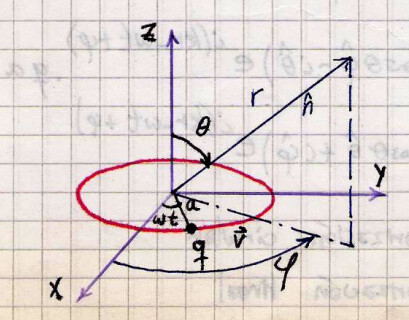
\includegraphics[width=0.3\textwidth]{images/fig_ft1_anillo_radiador.jpg} 
 
A partir del problema explicado en la figurita escribo $\vb{p}(t) = q \vbx(t)$ donde
\[
	\vbx = a [ \cos(\omega t)\xver + \sin(\omega t) \yver ]
\]
y será la física entonces extraíble desde $\text{Re}\{ \vb{p}_\omega \euler^{i\omega t}\}$.

Los elementos de la matriz $Q_{ij}$ son
\[
	Q_{xx} = q a^2 ( 3 \cos^2(\omega t) - 1 ) \qquad \qquad 
	Q_{yy} = q a^2 ( 3 \sin^2(\omega t) - 1 ) \qquad \qquad 
	Q_{zz} = - q a^2
\]
\[
	Q_{xy} = Q_{yx} = 3 q a^2 \cos(\omega t) \sin(\omega t) \qquad \qquad 
	Q_{xz} = Q_{yz} = Q_{zx} = Q_{zy} = 0
\]
Usando identidades trigonométricas usuales (pasar del cuadrado a uno solo y del producto
al seno del doble argumento) resulta el tensor separable en dos según
\[
	Q = 3 q \frac{a^2}{2} \begin{pmatrix}
	\cos( 2 \omega t ) & \sin( 2 \omega t ) &  0 \\
	\sin( 2 \omega t ) & -\cos( 2 \omega t ) &  0 \\
	0		&	0 	&	0 
	\end{pmatrix}
	+ q a^2
	\begin{pmatrix}
	\frac{1}{2} & 0 &  0 \\
	0 & \frac{1}{2} &  0 \\
	0		&	0 	&	-1
	\end{pmatrix}
\]
y considerando que $ Q = \text{Re}\left\{ Q_{2\omega}\euler^{ i \omega t } \right\}$ será
\[
	Q = 3 q \frac{a^2}{2} \begin{pmatrix}
	1 &  i &  0 \\
	i & -1 &  0 \\
	0 &  0 &  0 
	\end{pmatrix}
\]
de modo que 
\[
	\vb{A}_\text{dip}(t') = - \frac{i\omega}{cr}\vb{P}_\omega \euler^{-i\omega t'}
	\qquad \qquad 
	\vb{A}_\text{cuadrup}(t') = - \frac{2 \omega^2}{3c^2r} Q_{2\omega}\cdot\nver \euler^{-2i\omega t'}
\]
donde en esta última expresión, $\nver$ es el versor en coordenadas cartesianas según los ángulos
esféricos (ver Apéndice-esa cuenta la hicimos en el tomo de MC-).Luego,
\[
	Q_{2\omega}\cdot\nver = \frac{3}{2} q a^2 \sin\theta \euler^{i\vp}(\xver + i \yver )
\]
y hacemos la cuenta definiéndonos versores polares, ver ilustración, según
\[
	\xver = \cos\vp \rhover - \sin\vp \phiver
	\qquad 
	\yver = \sin\vp \rhover + \cos\vp \phiver
\]

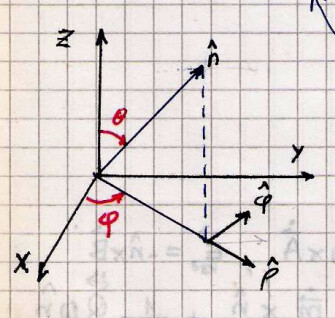
\includegraphics[width=0.3\textwidth]{images/fig_ft1_versoretes_polares.jpg} 

\[
	\nver \times (\xver + i\yver ) = 
	\rver \times [ ( \cos\vp + i\sin\vp )\rhover + i( \cos\vp + i\sin\vp )\phiver] =
	\euler^{i\vp}(\cos\theta \phiver - i \thetaver)
\]
Finalmente,
\[
	\vb{B}_\text{dip} = - \frac{1}{c} \frac{\omega^2}{cr} (\cos\theta \phiver - i \thetaver)
	q a \euler^{i(kr-\omega t+\vp)}
\]
\[
	\vb{E}_\text{dip} = \frac{\omega^2}{c^2r} (\cos\theta \phiver + i \thetaver)
	\euler^{i(kr-\omega t+\vp)}
\]
y tenemos casos
\[
	\begin{cases}
	\theta = 0 \qquad &\text{ polarización circular } \\
	\theta = {\pi}/{2} \qquad &\text{ polarización lineal } \\
	\theta \text{ genérico } \qquad &\text{ polarización elíptica} 
	\end{cases}
\]
que nos llevan a
\[
	\vb{B}_\text{cuad} = - \frac{i2}{c} \frac{qa^2\sin\theta \omega^3}{c^3r} (\cos\theta \phiver - i \thetaver)
	\euler^{2i(kr-\omega t+\vp)}
\]
y la polarización tiene los mismos valores que en el caso anterior.
 
\end{ejemplo}


\begin{ejemplo}{\bf Consulta pintorezca}

Las nubes (gotas de agua) dispersan en todas las frecuencias.
La $\sigma$ eficaz de Rayleigh va como $\omega^4$.
Tengamos en cuenta que es $\omega \ll \omega_0$ de modo que la longitud de onda de la luz
es mucho mayor que la longitud de onda de Larmor.

La pic muestra que se dispersa con gran eficacia las bajas longitudes de onda, de manera que el
azul se dispersa más.

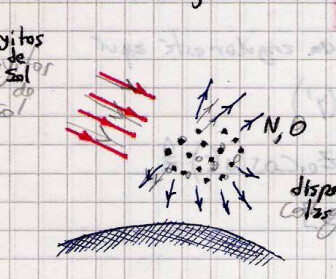
\includegraphics[width=0.4\textwidth]{images/fig_ft1_dispersion_sol.jpg}	

Cuando se pone el sol, se dispersa el azul y queda el rojo.
 
\end{ejemplo}


% =================================================================================================
\section{Frenado magnético}
% =================================================================================================

Sea la Figura; un disco conductor con espesor $d$ que gira.
Hacemos
\[
	\vb{E}' = \frac{1}{c}\pv{v}{B} = \omega \frac{r}{c} \hat{\phi} \times (-B\hat{z}) = 
	-\frac{\omega r B}{c} \hat{r}
\]
y la densidad de potencia disipada por corrientes de Foucault, por unidad de
volumen, será
\[
	\mathfrak{P} = \pe{P}{E'} = \sigma E'^2 = \frac{\sigma \omega^2 r^2 B^2}{c^2}
\]
donde la potencia total sale de integrar en todo el disco
\[
	P = \int \int \frac{\sigma \omega^2 r^2 B^2}{c^2} r d\theta dr =
		\frac{\sigma \omega^2 a^4 B^2 2\pi }{4 c^2}.
\]
Aunque yo anoté otro resultado en la carpeta, más con los dedos, que es
\[
	\frac{\sigma \omega^2 r^2 a^2 B^2 d }{c^2},
\]
para lo cual convendría mirar la figura (derecha).
Son corrientes de {\it Foucault} las que frenan el disco.

\begin{figure}[htb]
	\begin{center}
	\includegraphics[width=0.4\textwidth]{images/fig_ft1_frenado.pdf} 
	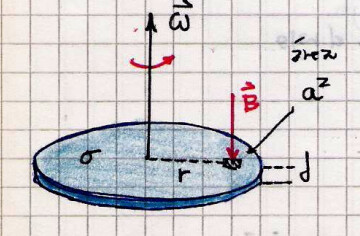
\includegraphics[width=0.4\textwidth]{images/fig_ft1_frenadoJPG.jpg}
	\end{center}
	\caption{}
\end{figure} 

En un disco fijo con $\vb{B} = B_0 \euler^{i\omega t}$  habrá $\vb{E} = E(r) \hat{\phi}$ de manera que 
$\pe{J}{E} = \sigma E(r)^2$ entonces se disipará energía por efecto Joule. Se calientan los 
transformadores en un ejemplo usual de la vida real.

Para compensar la pérdida de energía podemos aplicar un torque, que viene de $\pe{F}{v}$,
y es
\[
	\tau = \frac{\omega \sigma r^2 B^2 a^2 d }{c^2}.
\]

Otro caso es el de un disco conductor fijo. Ver ilustración. 

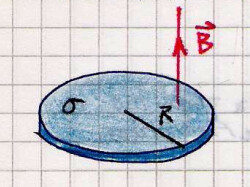
\includegraphics[width=0.25\textwidth]{images/fig_ft1_frenadoJPG2.jpg}

Tenemos un campo cuasiestacionario
\[
	\vb B = B_0 \sin(\omega t + \a) \zver
\]
luego desde la ecuación del rotor del campo eléctrico se tiene
\[
	\rotorm{E} = -\frac{1}{c} \dpar{\vb B}{t} = \frac{\omega B_0}{c} \sin(\omega t + \a) \zver 
\]
de lo cual deducimos que 
\[
	E_\vp = \frac{\omega}{2c} B_0r \sin(\omega t + \a) \phiver
\]
que aporta a $\vb J =\sigma\vb E$.
Se disipa energía por efecto Joule de esta forma.

La radiación requiere que $\vb E$ y $\vb B$ se retroalimenten o, como dice Feynman que se espoleen
mutuamente. Se consideran
\[
	\rotorm{E} = -\frac{1}{c}\dpar{\vb B}{t} \qquad 
	\rotorm{H} = \frac{1}{c}\dpar{\vb D}{t}
\]
con $\divem{B} = \divem{E} = 0$ de modo que $\vb B$ genera $\vb E$ y $\vb D$ genera $\vb H$; en un 
planteo cuasiestacionario despreciamos una variación temporal poer no las dos a la vez.

\begin{ejemplo}{\bf Problema 8}

Usaremos o queremos ve la fórmula de Larmor
\[
	P = \frac{2q^2}{3c^3} \Frac{d\vb v}{dt}^2
\]

En una órbita circular la partícula irradia

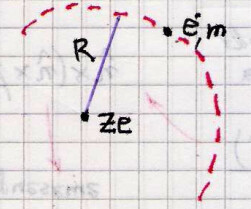
\includegraphics[width=0.2\textwidth]{images/fig_ft1_orbita_circular_particula.jpg}

Según la segunda ley de Newton,
\[
	|\dot{\vb v}| = \frac{v}{r} = \frac{Ze^2}{mR^2}
\]
y la potencia
\[
	P = \frac{2e^2Z^2e^4}{3c^3m^2R^4} = \dtot{\mathcal{E}}{t} = 
	- \dtot{}{t}\left( m \frac{v^2}{2} - \frac{Ze^2}{R} \right)=
	\dtot{}{t}\Frac{Ze^2}{2R},
\]
donde pensamos que el $R$ depende del tiempo.
\[
	P = - \dtot{\mathcal{E}}{R} \dtot{R}{t} = - \Frac{Ze^2}{2R} \dtot{R}{t} 
\]
y reemplazando cada cosa
\[
	\int_0^{\Delta t} -\frac{2Ze^4}{3m^2c^3} \: dt = \int_{R_0}^0 \frac{R^2}{2}dR,
\]
y entonces
\[
	\Delta t = \frac{m^2 c^3 R_0^3}{4Z} = \frac{R_0}{c} \Frac{R_0}{r_0}^2
\]
\notamargen{Estamos usando el radio clásico del electrón: $r_0 = e^2/(mc^2)$.}
Entonces,
\[
	c \Delta t \approx \frac{3}{Z} \text{ cm },
\]
y vemos que cuando el electrón decae la luz ha recorrido una distancia pequeña.
Realmente recorre una espiral en la cual va cayendo.
 
\end{ejemplo}


\subsection{Esponja electromagnética}

En $t=0$ se distribuye una $\sigma$ en la cara interna. Se genera una \vb{J} y un campo \vb{E} 
radial que no produce \vb{B} entonces $\vb{S}=0$ no hay radiación.


\begin{figure}[htb]
	\begin{center}
	\includegraphics[width=0.25\textwidth]{images/fig_ft1_esponja.pdf} 
	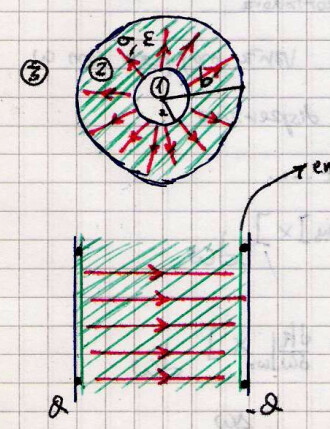
\includegraphics[width=0.25\textwidth]{images/fig_ft1_esponjaJPG.jpg}
	\end{center}
	\caption{}
\end{figure} 

La carga se mueve por el interior, se filtra por la zona gris, hasta llegar a la superficie y 
alcanzar situación estática $\vb{E}_{II} = 0$.
La energía disipada lo hace en forma de calor pero no se radía.

La energía final es menor pero no se escapó la energía.
Las tres zonas indicadas en la figurita se sucede lo siguiente
\[
	\begin{array}{cccc}
	& \textcircled{1} & \textcircled{2} & \textcircled{3} \\
	\hline \\
	t=0 & E_0 = 0 & E_1 = \frac{Q}{\epsilon r^2} & E_3 =\frac{Q}{r^2} \\
	& & & \\
	t\to\infty & E_0 = 0 & E_1 = 0 & E_3 = \frac{Q}{r^2}  
	\end{array}
\]

Para una capacitor se tiene que en $t=0$ se larga las tapas y se empiezan a descargar las
chapas del mismo.
\[
	W_{t=0} = \int_a^b + \int_b^\infty \qquad 
	W_f = \int_b^\infty \qquad W_f < W_{t=0}
\]

En algún caso se tiene de la ecuación del rotor de $\vb B$
\[
	\left( \dpar{}{t} + \frac{4\pi\sigma}{\varepsilon} \right) E_r = 0 
\]
y
\[
	E_r = E_0 \euler^{- 4\pi\sigma/\varepsilon t},
\]
el campo eléctrico decae con el tiempo de relajación. Y si la $\vb J = \sigma \vb B$ se tiene
\[
	\int_a^b \int_{t=0}^{t=\infty} \sigma |\vb E|^2 \: dt \: dV = 
	\text{Energía disipada}
\]

\subsection{Pulso EM que se propaga}

Consideramos que todas las componentes tienen la misma amplitud en el intervalo
de frecuencias dado por $|\omega - \omega_0|<\Delta\omega/2$

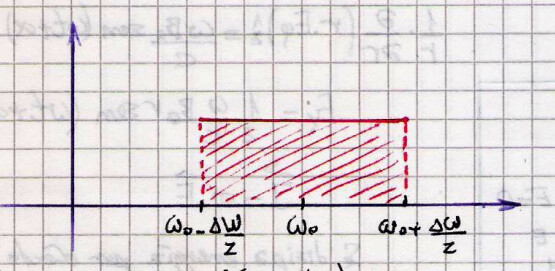
\includegraphics[width=0.45\textwidth]{images/fig_ft1_pulso_em1.jpg}

Luego,
\[
	E = \int E(\omega) \euler^{i(\omega t - kx )} \: d\omega =
	E_0 \int_{\omega_0-\Delta\omega/2}^{\omega_0+\Delta\omega/2} 
	\euler^{i(\omega t - kx )} \: d\omega
\]
y tenemos la relación $\Delta \omega \ll \omega_0 $ que nos dice que el ancho de banda
es mucho menor que la frecuencia de la portadora.
$k=k(\omega)$ pero varía muy poco; es un medio poco dispersivo, entonces soporta una 
expansión de Taylor,
\[
	k(\omega) = k(\omega_0) + \left. \dtot{k}{\omega}\right|_{\omega_0}(\omega -\omega_0) +
	...
\]

Los casos usuales serían que si $k=\omega/c$ el pulso se propaga sin deformarse, aka 
dispersión nula; en cambio si $k=f(\omega)$ tenemos dispersión y deformación.

\[
	E = E_0 \int_{\omega_0-\Delta\omega/2}^{\omega_0+\Delta\omega/2} 
	\euler^{i(\omega t - [k_0 + (\omega-\omega_0)dk/d\omega|_{\omega_0} ] \: x )} \: d\omega,
\]
pero esta integral se puede hacer y resulta
\[
	E = E_0 \euler^{-i(\omega_0 t - k_0x )} 
	\left( 
	\left. \frac{ \euler^{-i u ( t - dk/d\omega|_{\omega_0} x ) } }{ t - dk/d\omega|_{\omega_0} x} 
	\right|_{-\Delta\omega/2}^{\Delta\omega/2}
	\right)
\]
\[
	E = E_0 \euler^{-i(\omega_0 t - k_0x )} 
	\frac{ 2 \sin\left( t - dk/d\omega|_{\omega_0} x \Delta\omega/2 \right) }
	{ t - dk/d\omega|_{\omega_0} x } 
\]
y se tiene $t = dk/d\omega|_{\omega_0} x$ que es la velocidad de grupo (la velocidad a la cual
se propaga la energía).
Tenemos la relación de incertidumbre, $\Delta \omega \Delta t \geq 1/2$, que es del orden de
$2\pi$.


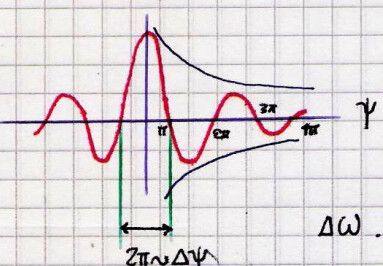
\includegraphics[width=0.45\textwidth]{images/fig_ft1_pulso_em2.jpg}



\begin{ejemplo}{\bf Problema 1: dispersión de Thomson}

Tenemos el siguiente esquema con coordenadas. Existe un campo eléctrico $\vb E$ oscilante, que
hará oscilar al electrón.
Se puede calcular por potenciales de Lienard-Wiechert

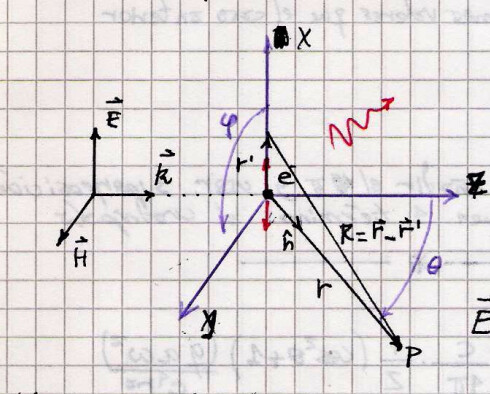
\includegraphics[width=0.25\textwidth]{images/fig_ft1_proble_thomson1.jpg}

Usaremos la fórmula usual para el $\vb E_\text{rad}$ y el campo magnético de radiación saldrá
del vectorial y evaluar en $t'$. Tomaremos
\[
	t' = t - \frac R c \approx t - \frac r c
\]
donde no consideramos coseno del ángulo porque no hay términos de interferencia.
Tendremos en cuenta polarización lineal y para las ecuaciones de movimiento despreciaremos la
parte de fuerza que hace el campo magnético, de manera que
\[
	m\ddot{x} = -e E_0 \euler^{i(kz-\omega t)} \qquad 
	m c \dot{\beta} = -e E_0 \euler^{i(kz-\omega t)} = -e E_0 \cos(\omega t)
\]

No recibe impulso, entonces no se desplaza en $\zver$ como la velocidad es baja hacemos el 
cálculo no relativista. Luego,
\[
	\vb{E}_\text{rad} \approx \frac{e}{c} \frac{\nver \times (\nver \times \dot{\vb{\beta}})}{R}
\]
donde $\nver$ es el esférico, de manera que, luego de un rato,
\[
	\nver \times (\nver \times \dot{\vb{\beta}}) =
	-\frac{eE_0}{mc}\cos(\omega t)
	\left[ 
	-( 1 - \sin^2\theta \cos^2\vp )\xver + 
	\sin^2\theta \sin\vp \cos\vp \yver + 
	\sin\theta \cos\theta \cos\vp \zver
	\right]
\]
y se tiene 
\[
	\vm{\pe{S}{\nver}} = \frac{c}{8\pi r^2} \Frac{E_0 e^2}{mc^2}^2( 1 - \sin^2\theta \cos^2\vp )
\]

Parto de $E_x$, si quiero cp debo sumarle una componente en $\yver$ desfasada en $i$. Luego,
\[
	\hat{e} = \frac{\xver + i\yver }{\sqrt{2}}
\]

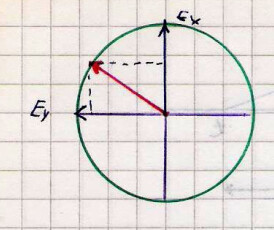
\includegraphics[width=0.25\textwidth]{images/fig_ft1_proble_thomson2.jpg}
 
De manera que resultan ambos iguales
\[
	\vm{\dtot{P}{\Omega}}_x = \frac{c}{8\pi}\Frac{ e^2 E_0}{ \sqrt{2} m c^2 }^2 
	( 1 - \sin^2\theta \cos^2\theta ) = \vm{\dtot{P}{\Omega}}_y.
\]

Superponiendo el campo $E$, no la potencia $P$, i.e. considero un campo $ \vb{E} = 2^{-1/2}
( E\xver + i E \yver ) $ se tiene 
\[
	\vm{\dtot{P}{\Omega}} = \vm{\dtot{P}{\Omega}}_x + \vm{\dtot{P}{\Omega}}_y =
	\frac{c}{8\pi} \Frac{E_0e^2}{mc^2}^2 \Frac{1+\cos^2\theta}{2}
\]
y consecuentemente,
\[
	\dtot{\sigma}{\Omega} = \vm{\dtot{P}{\Omega}} / \vm{S}_\text{inc} =
	\Frac{e^2}{mc^2}^2 \Frac{1+\cos^2\theta}{2}
\]
y normalizamos de alguna manera la potencia por ángulo sólido habiendo dividido por 
$ \vm{S}_\text{inc} = c/(8\pi) E_0^2$.

Si integramos en ángulo sólido resulta
\[
	\sigma_T = \frac{8\pi}{3}R^2_e,
\]
que es aproximadamente la sombra.

Notemos que para cálculo relativista tendremos un efecto Compton con cambio de longitud de onda
con lo cual debemos corregir 
\[
	\dtot{\sigma}{\Omega}\Frac{K'}{K}
\]
y
\[
	\frac{K'}{K} = \frac{1}{\displaystyle 1 + \frac{\hbar\omega}{mc^2}(1-\cos\theta)}.
\]

Si la partícula estuviera ligada a un potencial, deberá figurar en la ecuación de movimiento
\[
	m\ddot{x} + m \omega_0^2x = -e E_0 \cos(\omega t)
\]
\[
	x = - \frac{e E_0}{\omega_0^2 - \omega^2} \euler^{i\omega t}
\]
de manera que ahora tendremos
\[
	\sigma = \frac{8\pi}{3}\Frac{e^2}{mc^2}^2 \frac{\omega^4}{[\omega_0^2 - \omega^2]^2},
\]
y con frecuencia baja se recuperea el $\sigma$ de Thomson. Por otra parte si la frecuencia
es mucho menor, i.e. si $\omega \ll \omega_0$ se tiene el interesante resultado
\[
	\sigma = \sigma_T \Frac{\omega}{\omega_0}^4.
\]

\end{ejemplo}

% \bibliographystyle{CBFT-apa-good}	% (uses file "apa-good.bst")
% \bibliography{CBFT.Referencias} % La base de datos bibliográfica

\end{document}
